\documentclass[11pt,letterpaper]{article}
\input{headings}
\newcommand \recipeName {Fish with Essaouira Chermoula}
\newcommand \fileName {FishWithEssaouiraChermoula}
\chead{\recipeName}

\begin{document}
\input{title}

Chermoula is a a marinate of herbs and spices and lemon that Moroccans usually have with fish. There are many versions of Chermoula. This one is from the city of Essaouira. My modification is to add Pimenta de Cheiro, a fragrant, not so hot, pepper from Brazil. Several alternative Chermoulas mention the use of a pepper that is not too hot. Just as I was researching this recipe, I read a note on Cook's Illustrated (September/October 2018, page 5) about how an enzyme in garlic, alliinaze, converts a chemical compound in garlic, alliin, into another pungent compound, allicin, within thirty seconds of the garlic being cut. Quickly adding an acid to the garlic prevents this reaction, keeping the garlic mild. You want the milder garlic flavour in this fish dish. Thus speed is important when mixing the garlic with the lemon. 

\begin{description}

\item[Ingredients:]\ \\
	\begin{itemize}
	\item 1 teaspoon of cumin 
	\item 1/2 teaspoon of coriander
	\item 1 teaspoon of paprika
	\item 2 pimenta de cheiro
	\item 1 teaspoon of salt or to taste
	\item 3 cloves of garlic, peeled
	\item 2 tablespoons of freshly squeezed lemon juice
	\item 4 tablespoons of chopped fresh flat-leaf parsley
	\item 4 tablespoons of olive oil
	\item 4 pieces of cod fillet
	\end{itemize}

\item[Procedure:]\ \\
	\begin{enumerate}
	\item {\bf Toast and grind spices:}
		\begin{itemize}
		\item Cut a relatively small rectangle of parchment paper, make a folder in the paper and put it on the counter.
		\item Place cumin and coriander in a dry skillet.
		\item Place skillet over moderate heat and toast the seeds until they are fragrant.
		\item Immediately transfer the toasted spices to the paper.
		\item Use the folder to dump the spices into a coffee grinder or spice grinder.
		\item Grind the spices into a powder.
		\item If there are large pieces of shells from the coriander, you may need to sift the ground spices to remove them.
		\end{itemize}
	\item {\bf Prepare the Chermoula:}
		\begin{itemize}
		\item Squeeze the lemon juice and strain the seeds into a small bowl.
		\item Place the garlic on the cutting board. 
		\item Crush the garlic with  a chef's knife.
		\item Acting quickly, add the the salt to the garlic and crush into a paste.
		\item Transfer the garlic paste to the small bowl of lemon juice and use a small spoon to stir well as soon as you can.
		\item Cut the pimenta de cheiro into a pulp and add to the bowl
		\item Cut the parsley into a very fine chop and add to the bowl.
		\item Dump the ground spices and the paprika into the bowl.
		\item Stir well
		\end{itemize}
	\item {\bf Marinate the fish}
		\begin{itemize}
		\item About two hours before cooking dry the fish fillets well with paper towels.
		\item Rub the Chermoula onto the fish.
		\item Cover the fish with a foil and let seat, at room temperature, for two hours.
		\end{itemize}
	\item {\bf Saute the fish}
		\begin{itemize}
		\item Warm a serving platter either in the oven or with hot water.
		\item Heat up a non-stick skillet until fairly hot and pour enough olive oil to just cover the bottom. 
		\item Saute the fish making sure that it is undercooked. If making a large amount, it is specially important to undercook the initial batch as the fish continues cooking after it is removed from the pan and other hot pieces are put on top.
		\item As soon as each piece is done, remove to the warm serving platter.
		\item Pour any sauce that formed in the pan or remaining olive oil in the pan over the fish.
		\item Serve immediately
		\end{itemize}
	\end{enumerate}
\end{description}
\begin{table}
\begin{tabular}{cccc}
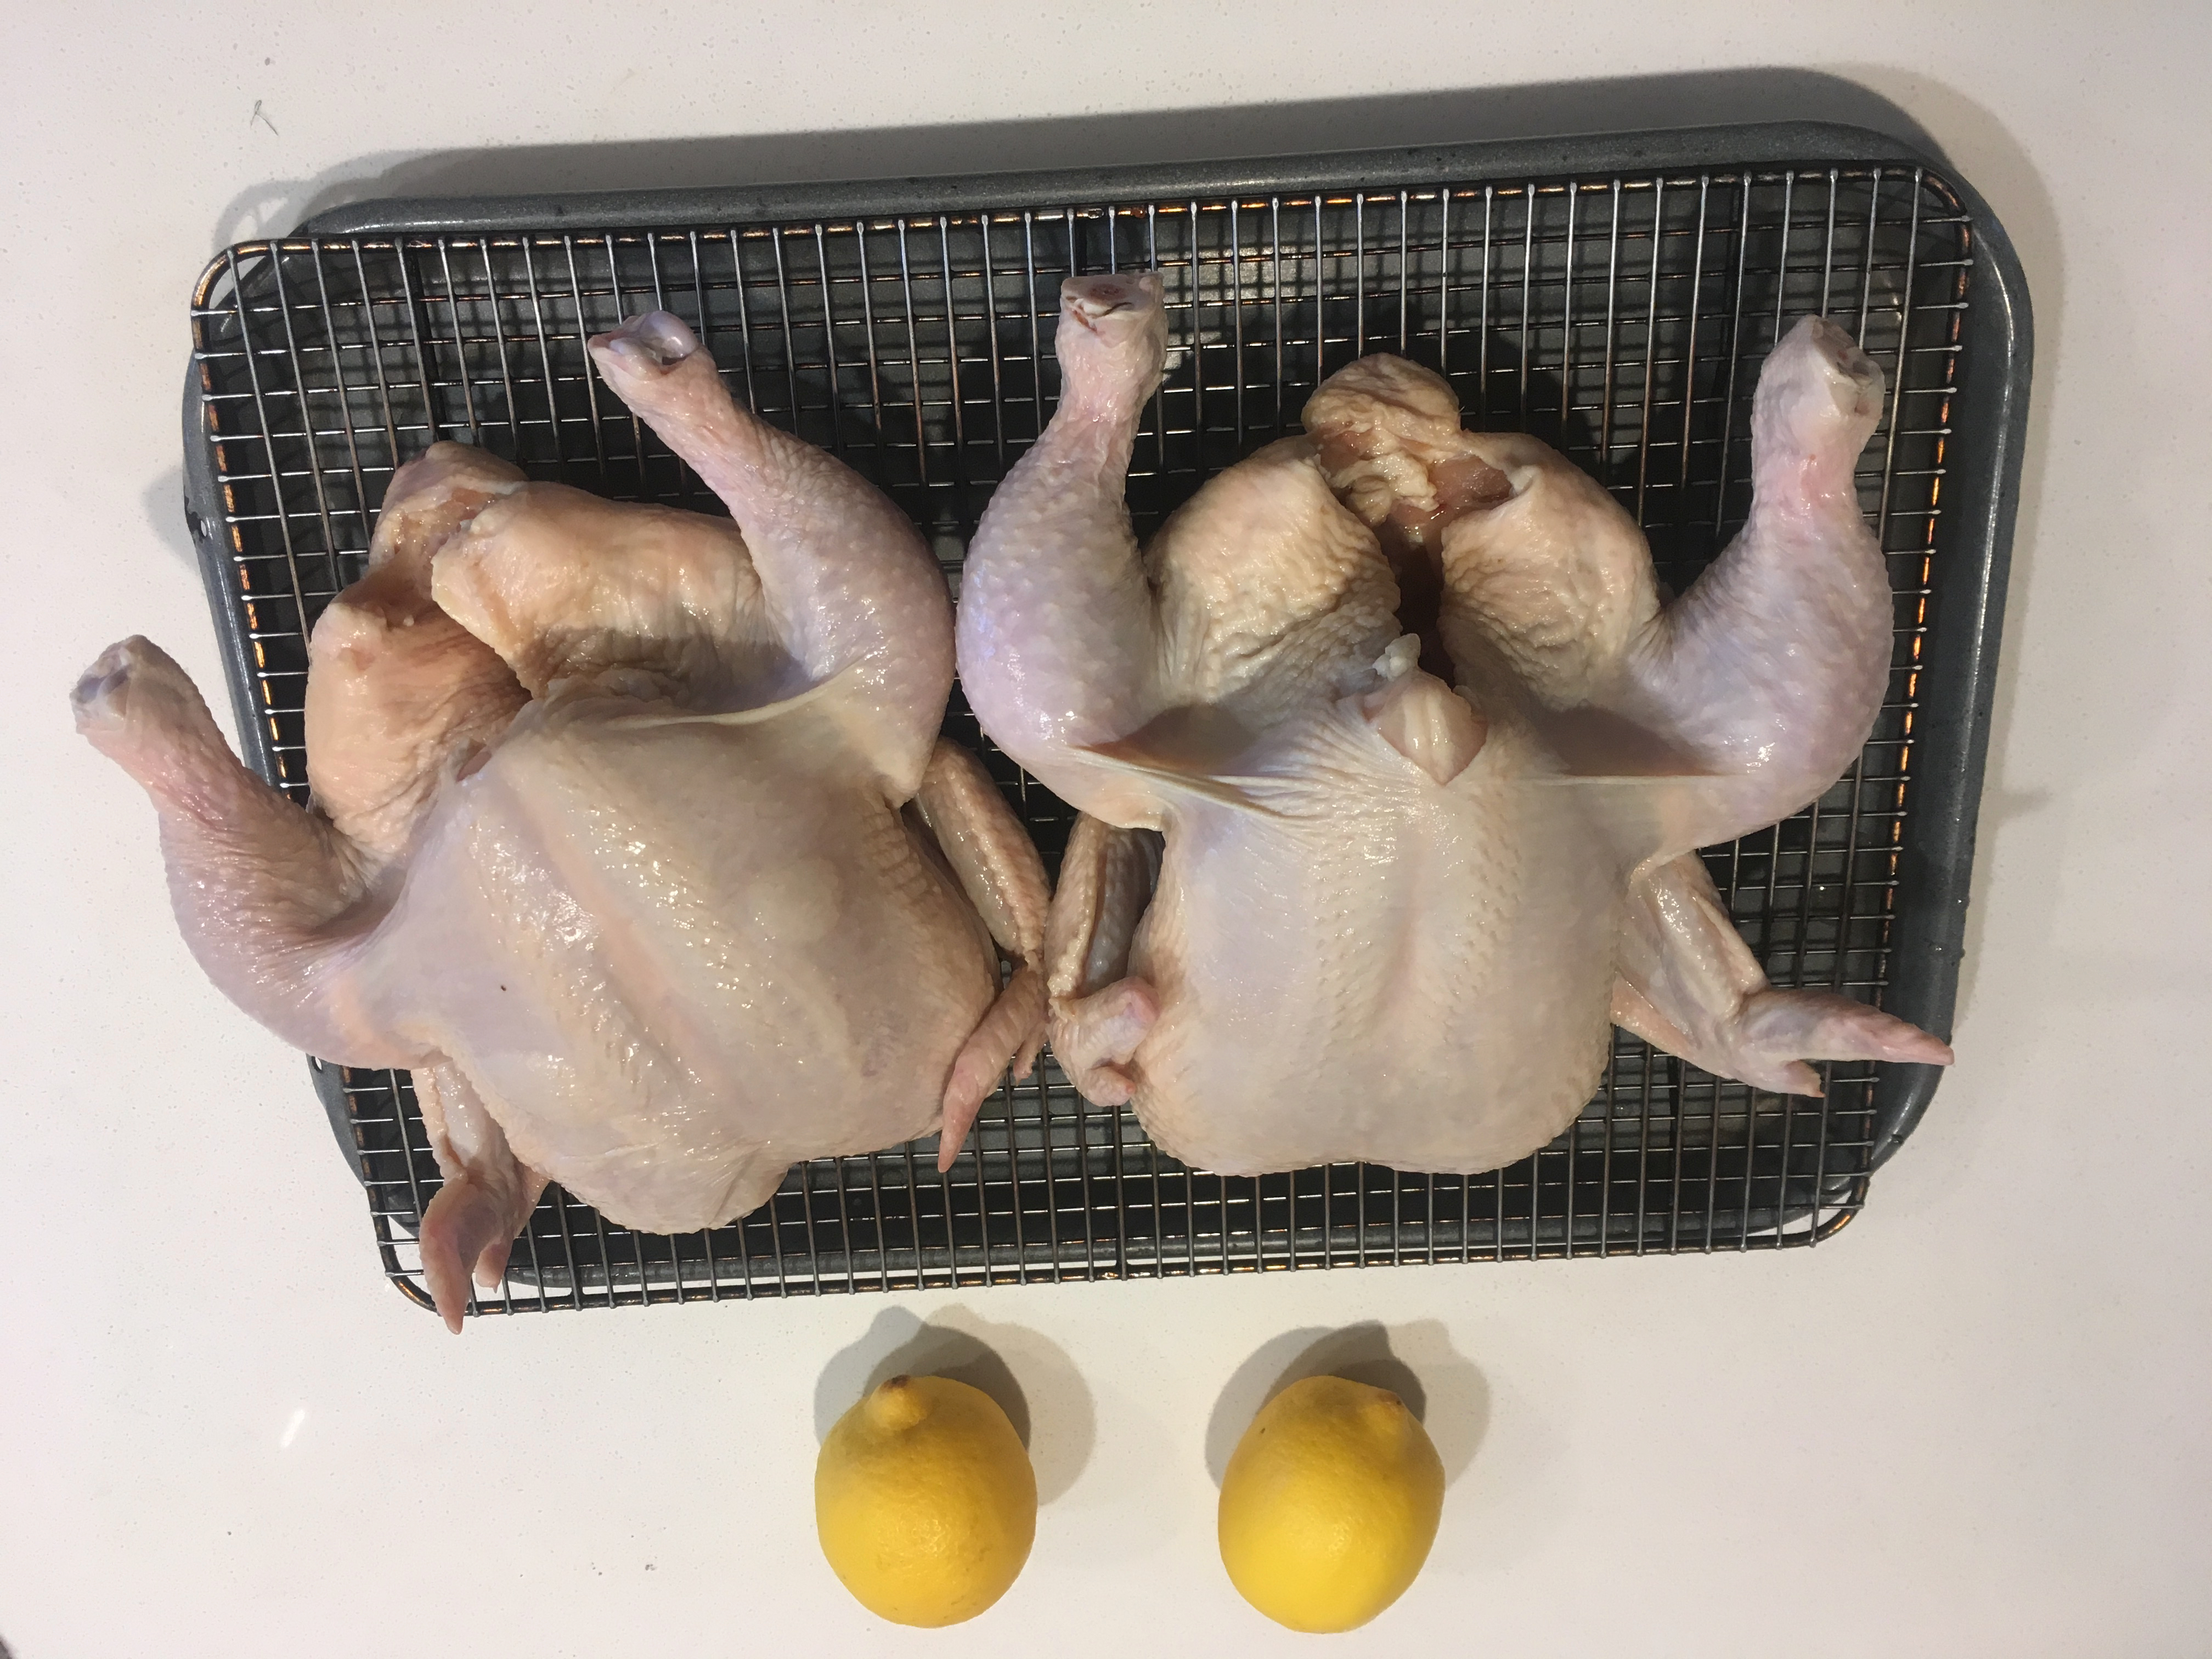
\includegraphics[width=0.25\textwidth]{\imageDir/\fileName/IMG_3197.jpg} &
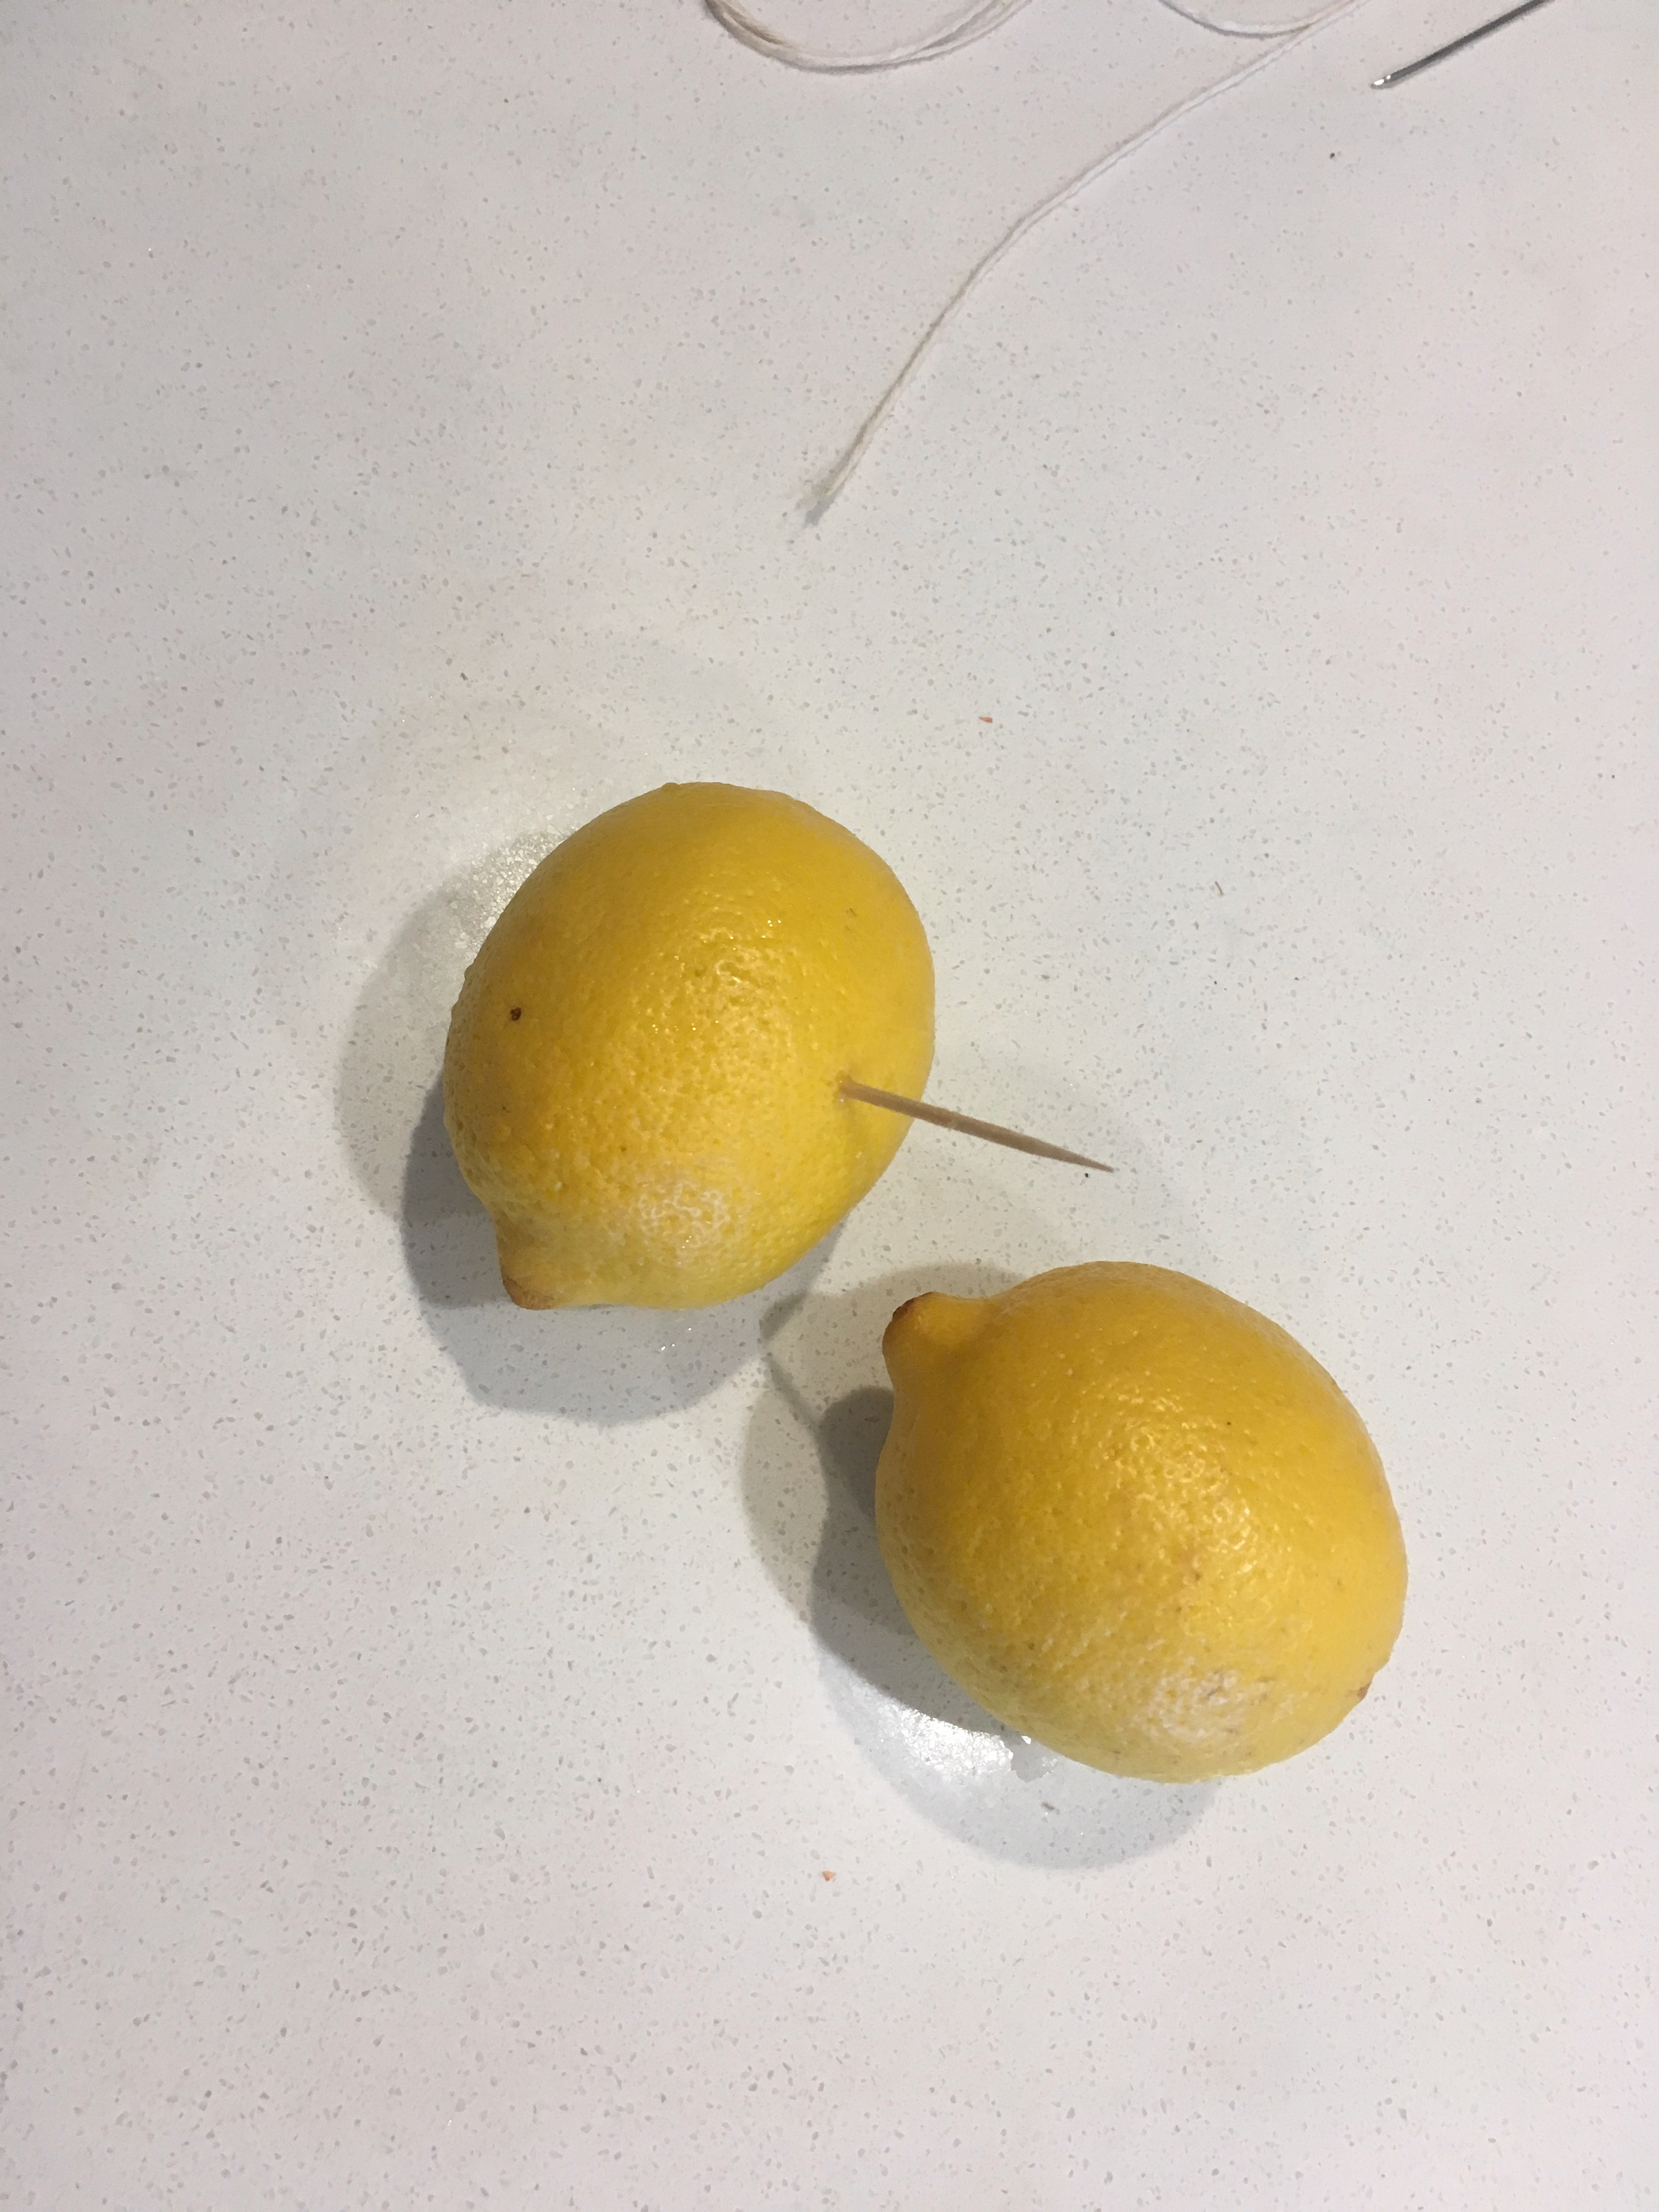
\includegraphics[width=0.25\textwidth]{\imageDir/\fileName/IMG_3212.jpg} &
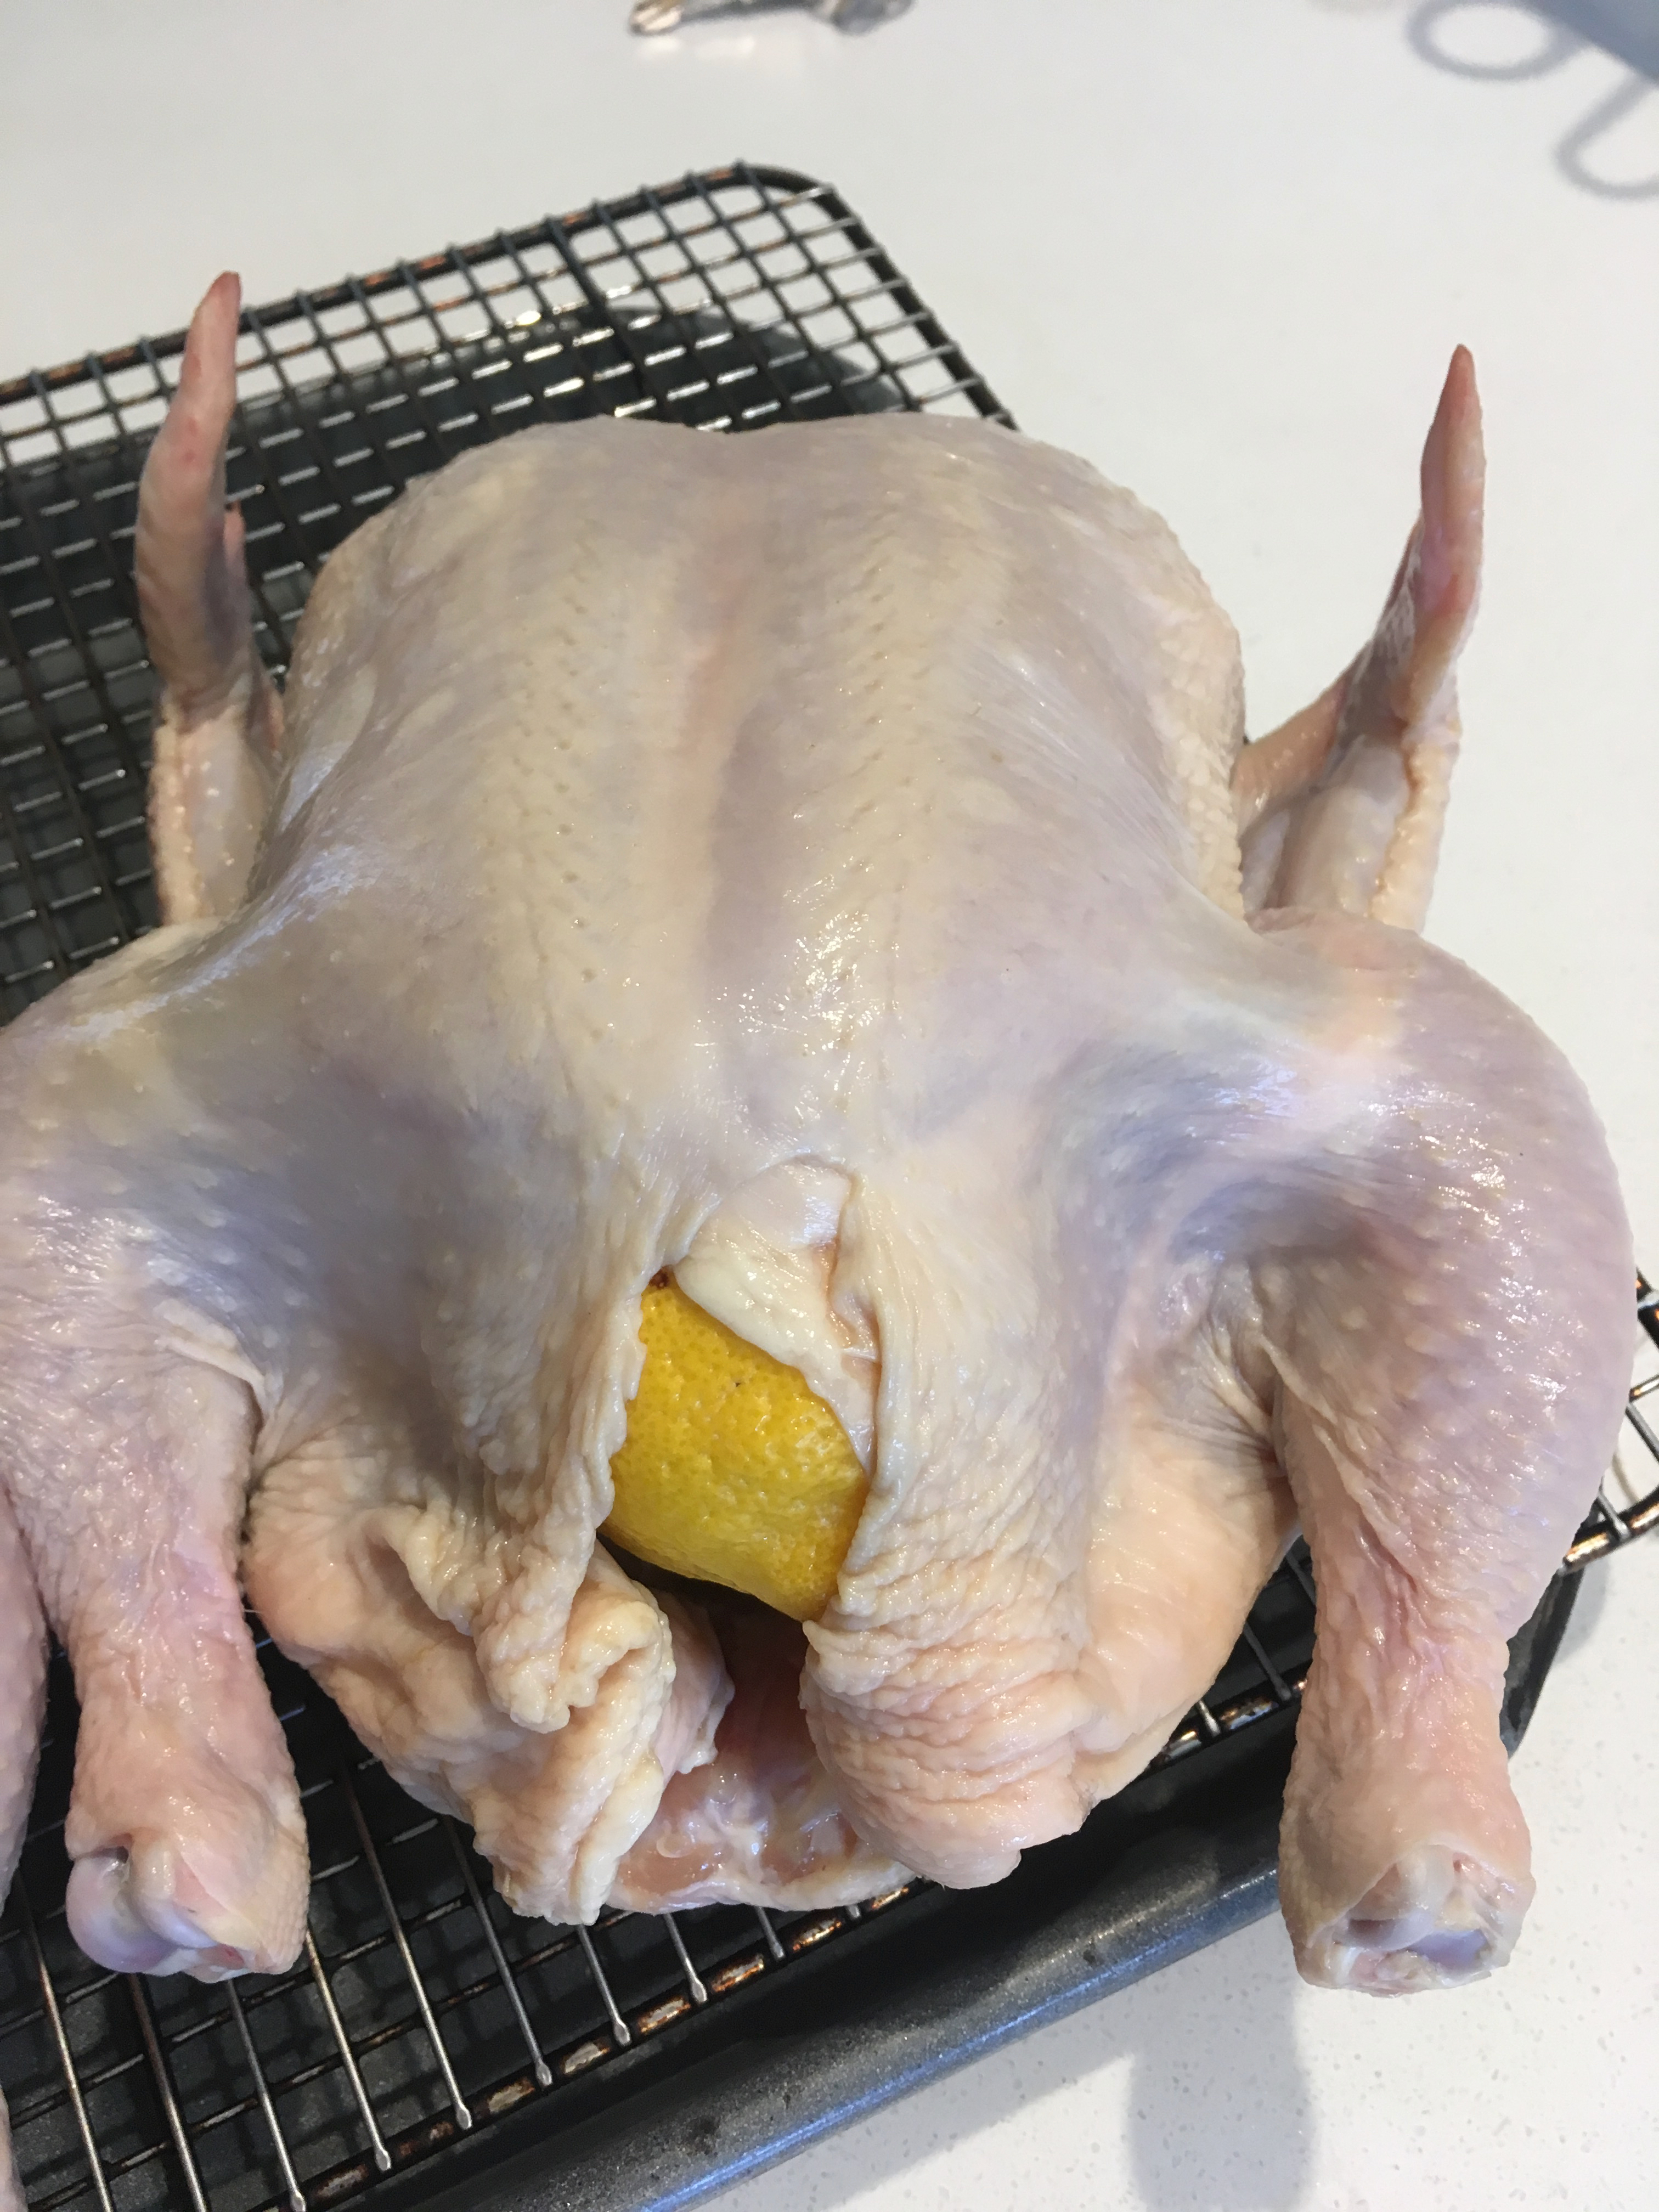
\includegraphics[width=0.25\textwidth]{\imageDir/\fileName/IMG_3213.jpg} \\
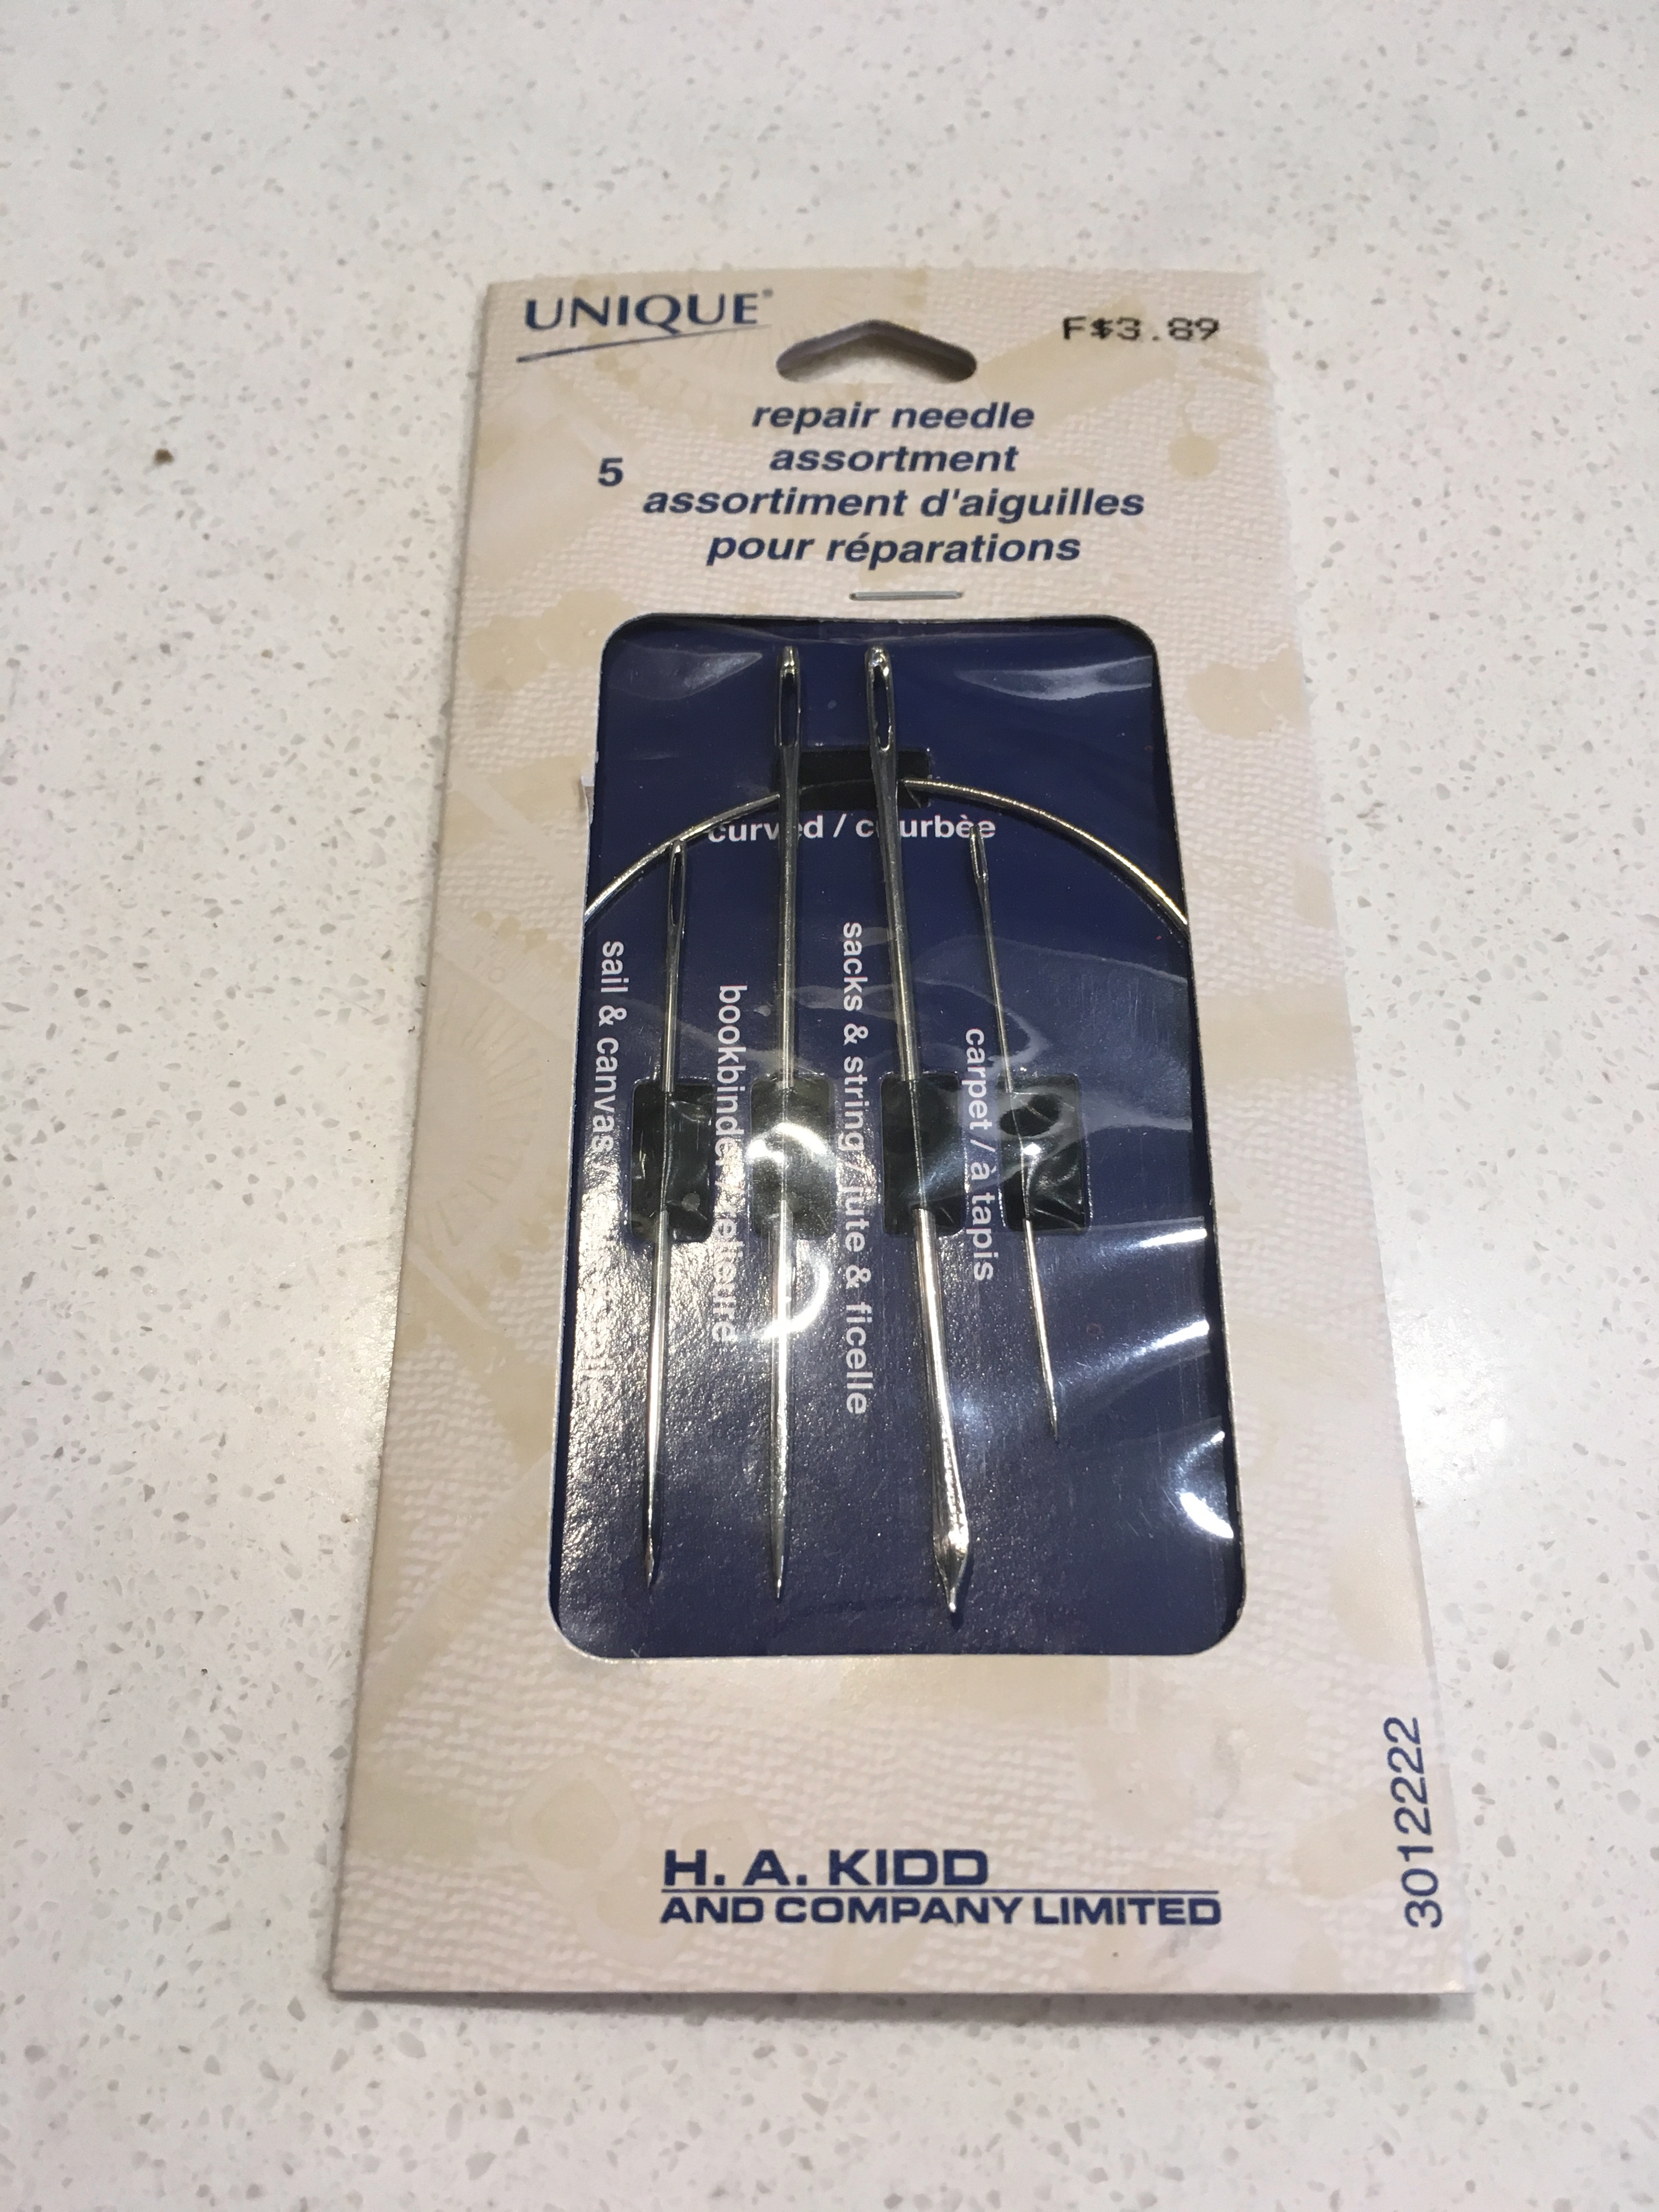
\includegraphics[width=0.25\textwidth]{\imageDir/\fileName/IMG_3206.jpg} &
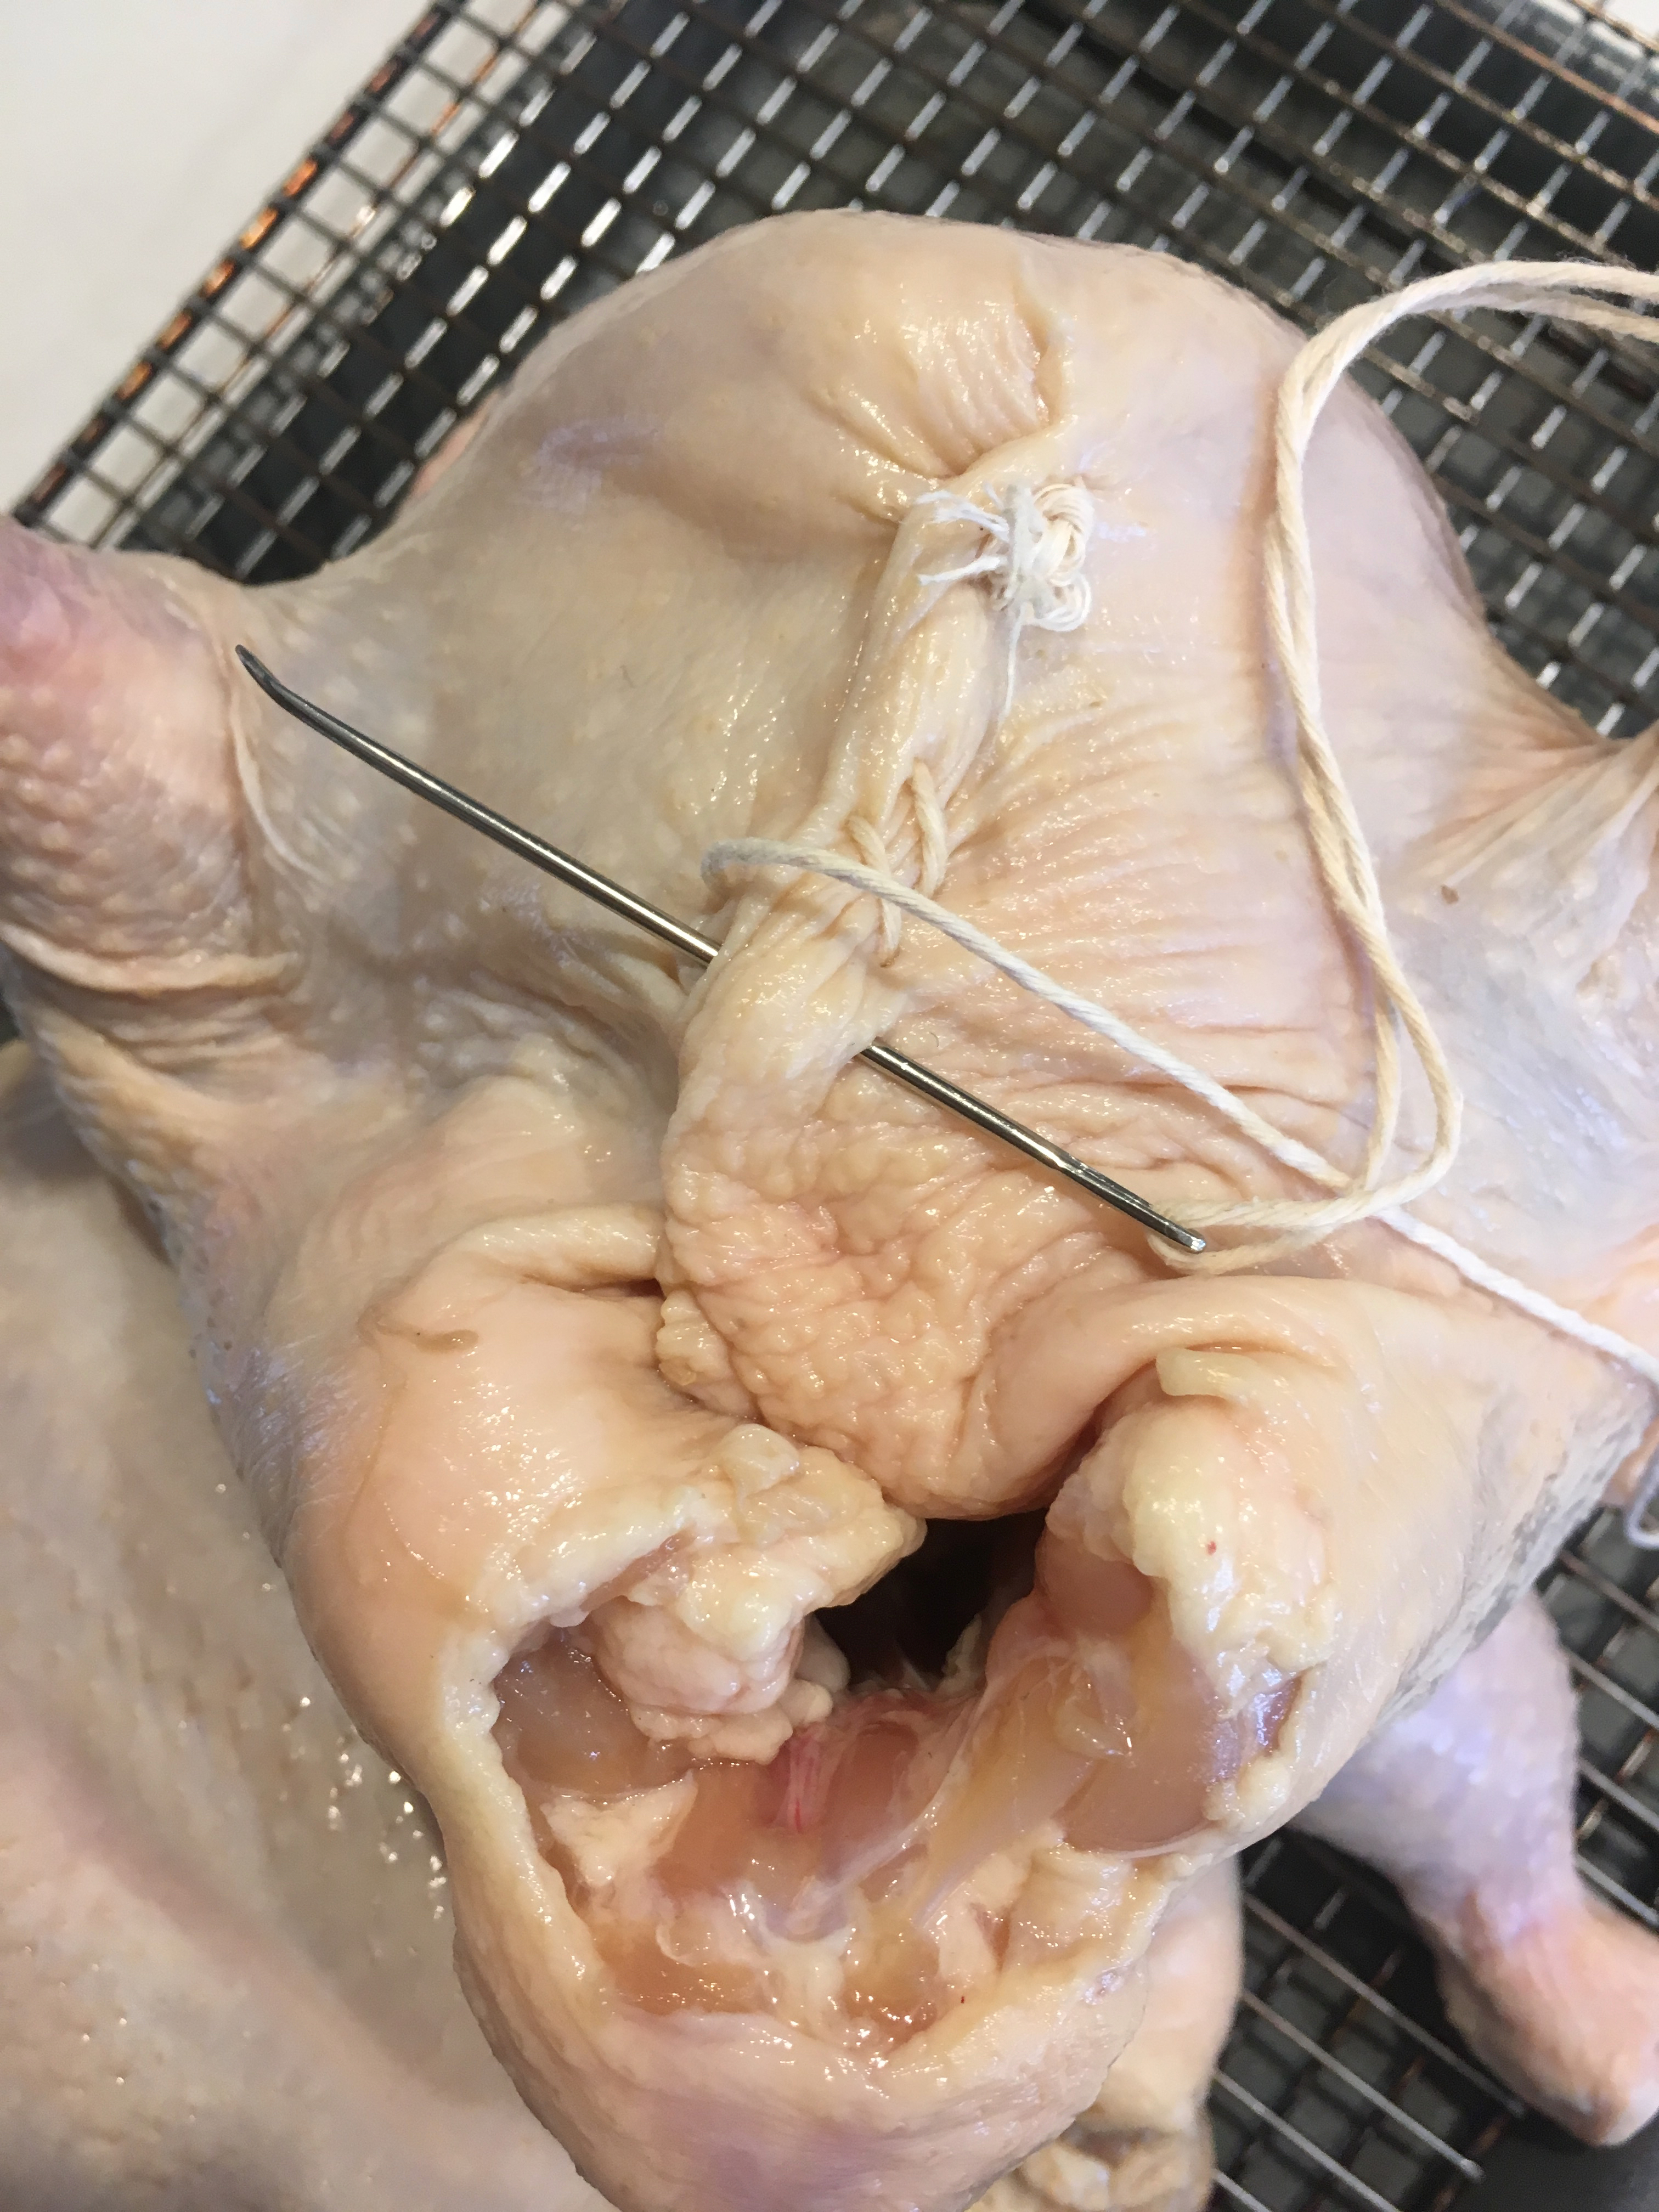
\includegraphics[width=0.25\textwidth]{\imageDir/\fileName/IMG_3214.jpg} &
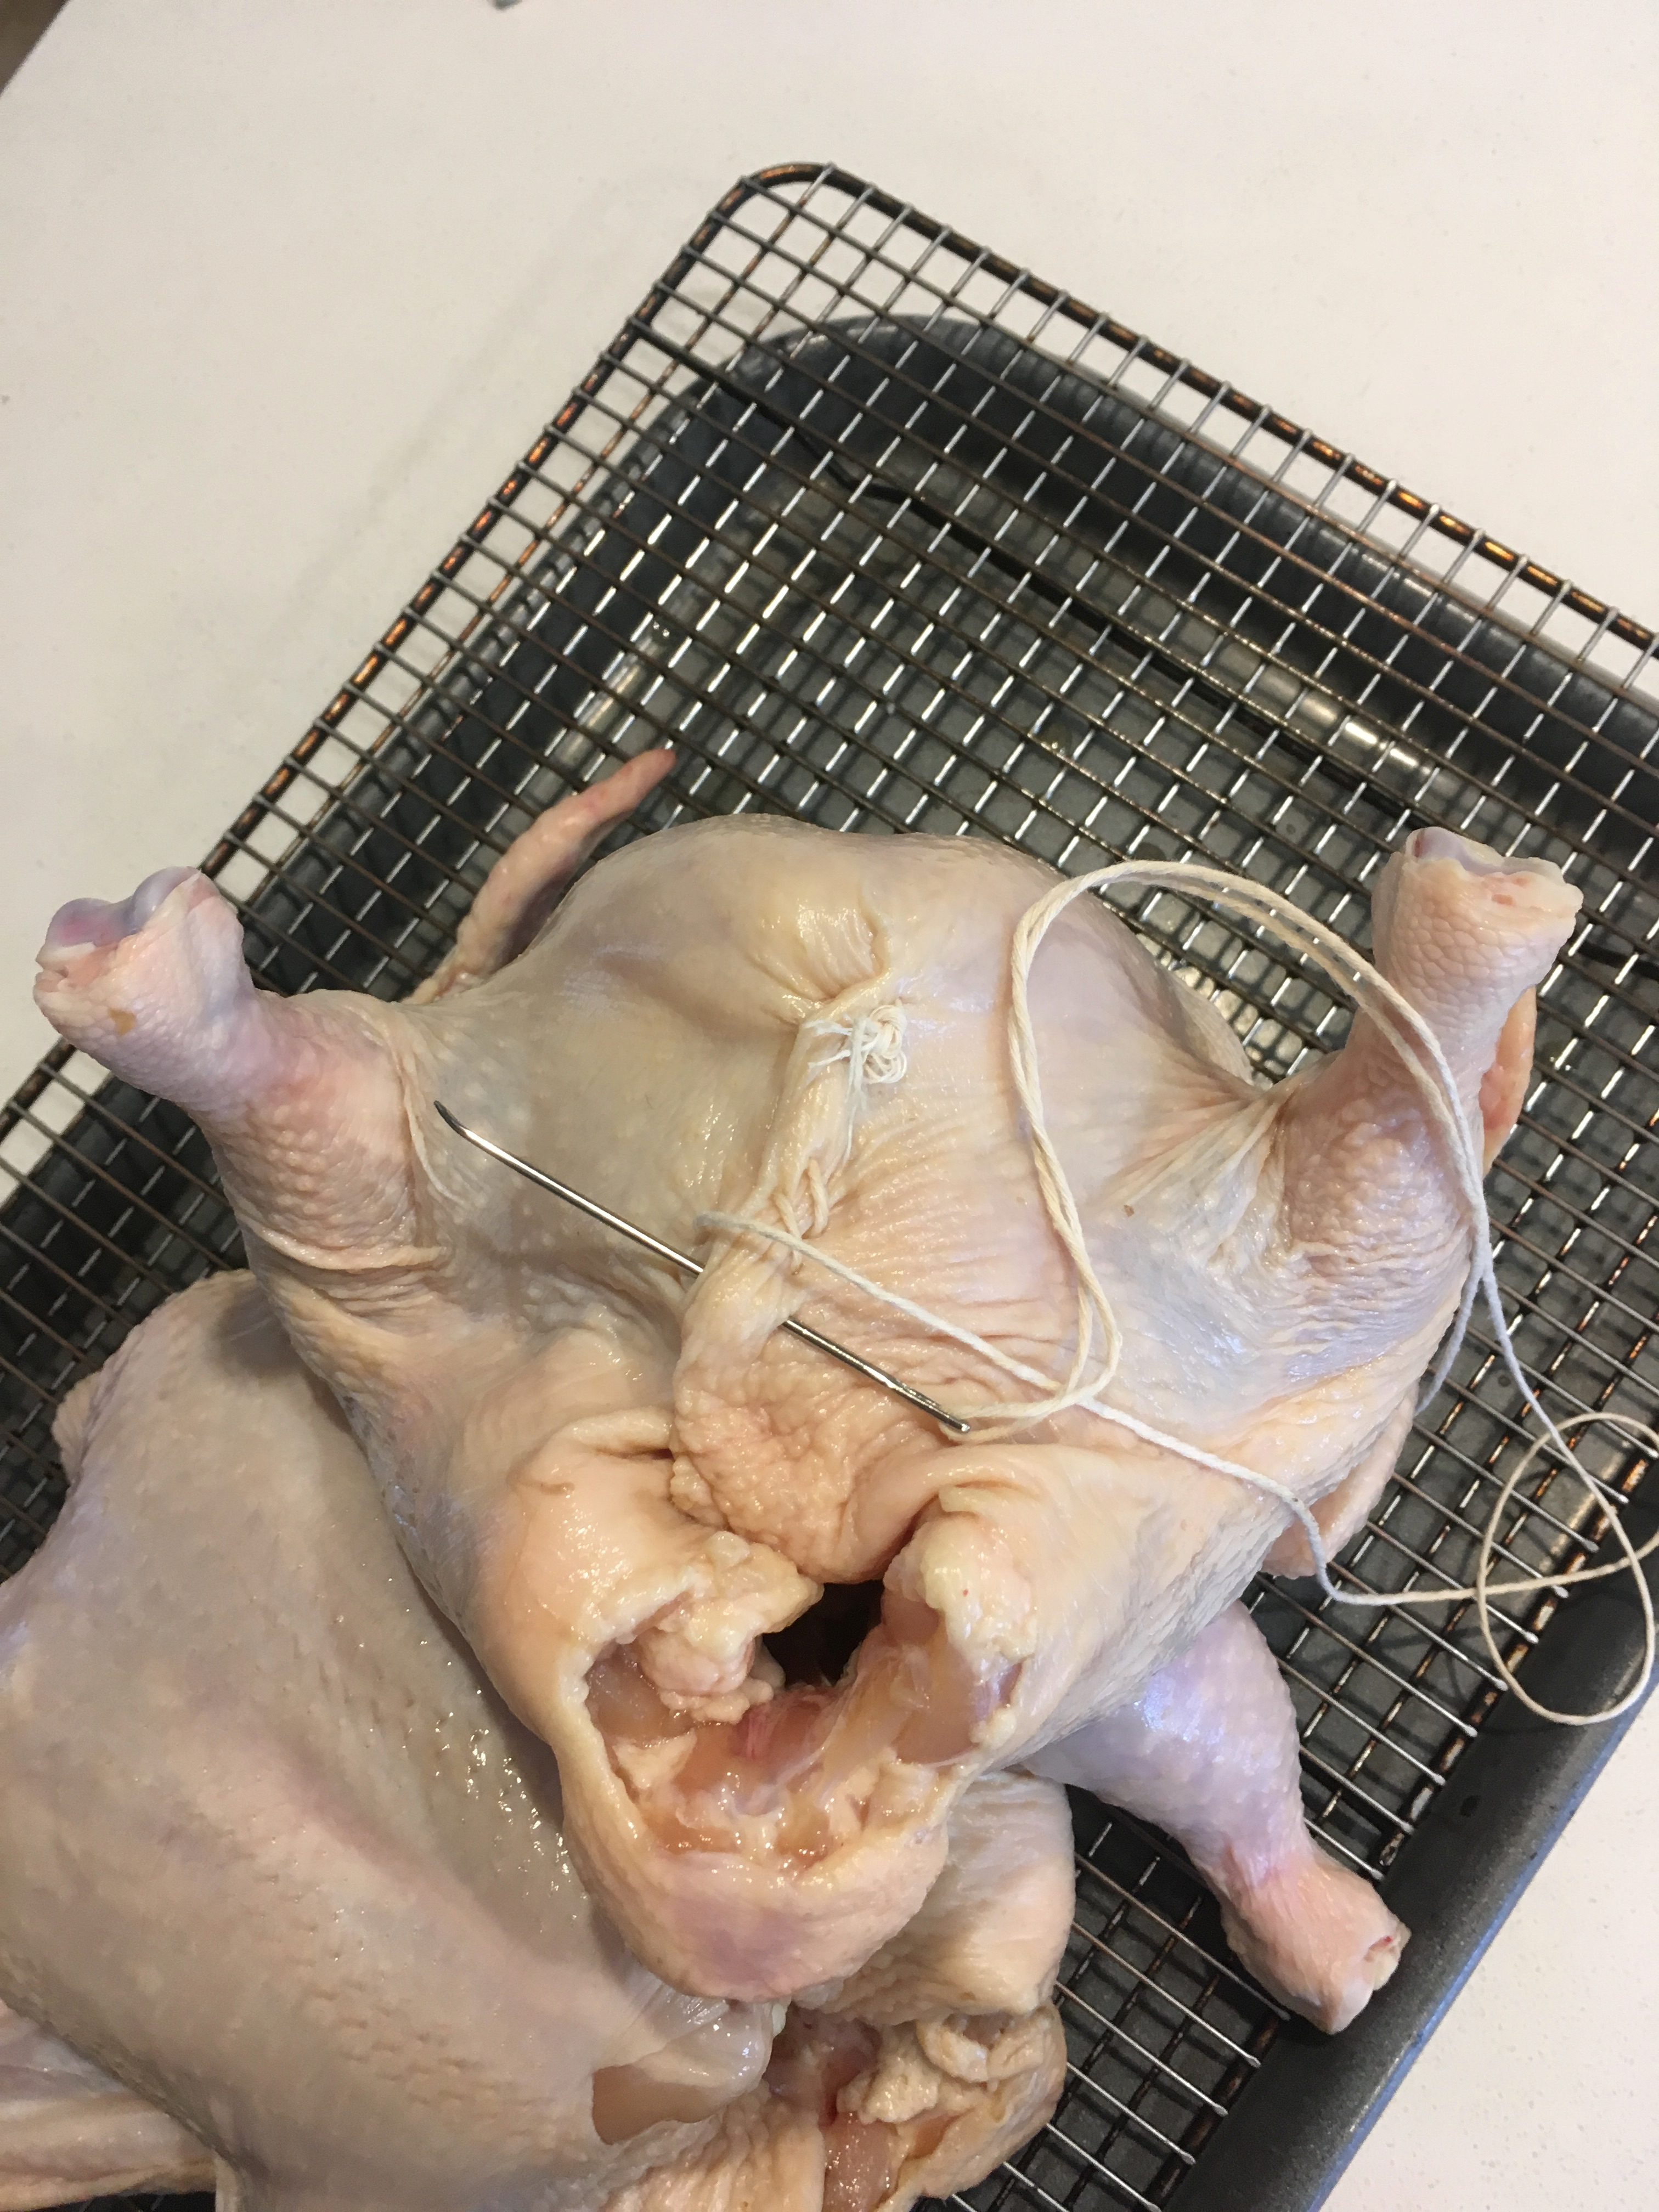
\includegraphics[width=0.25\textwidth]{\imageDir/\fileName/IMG_3216.jpg} \\
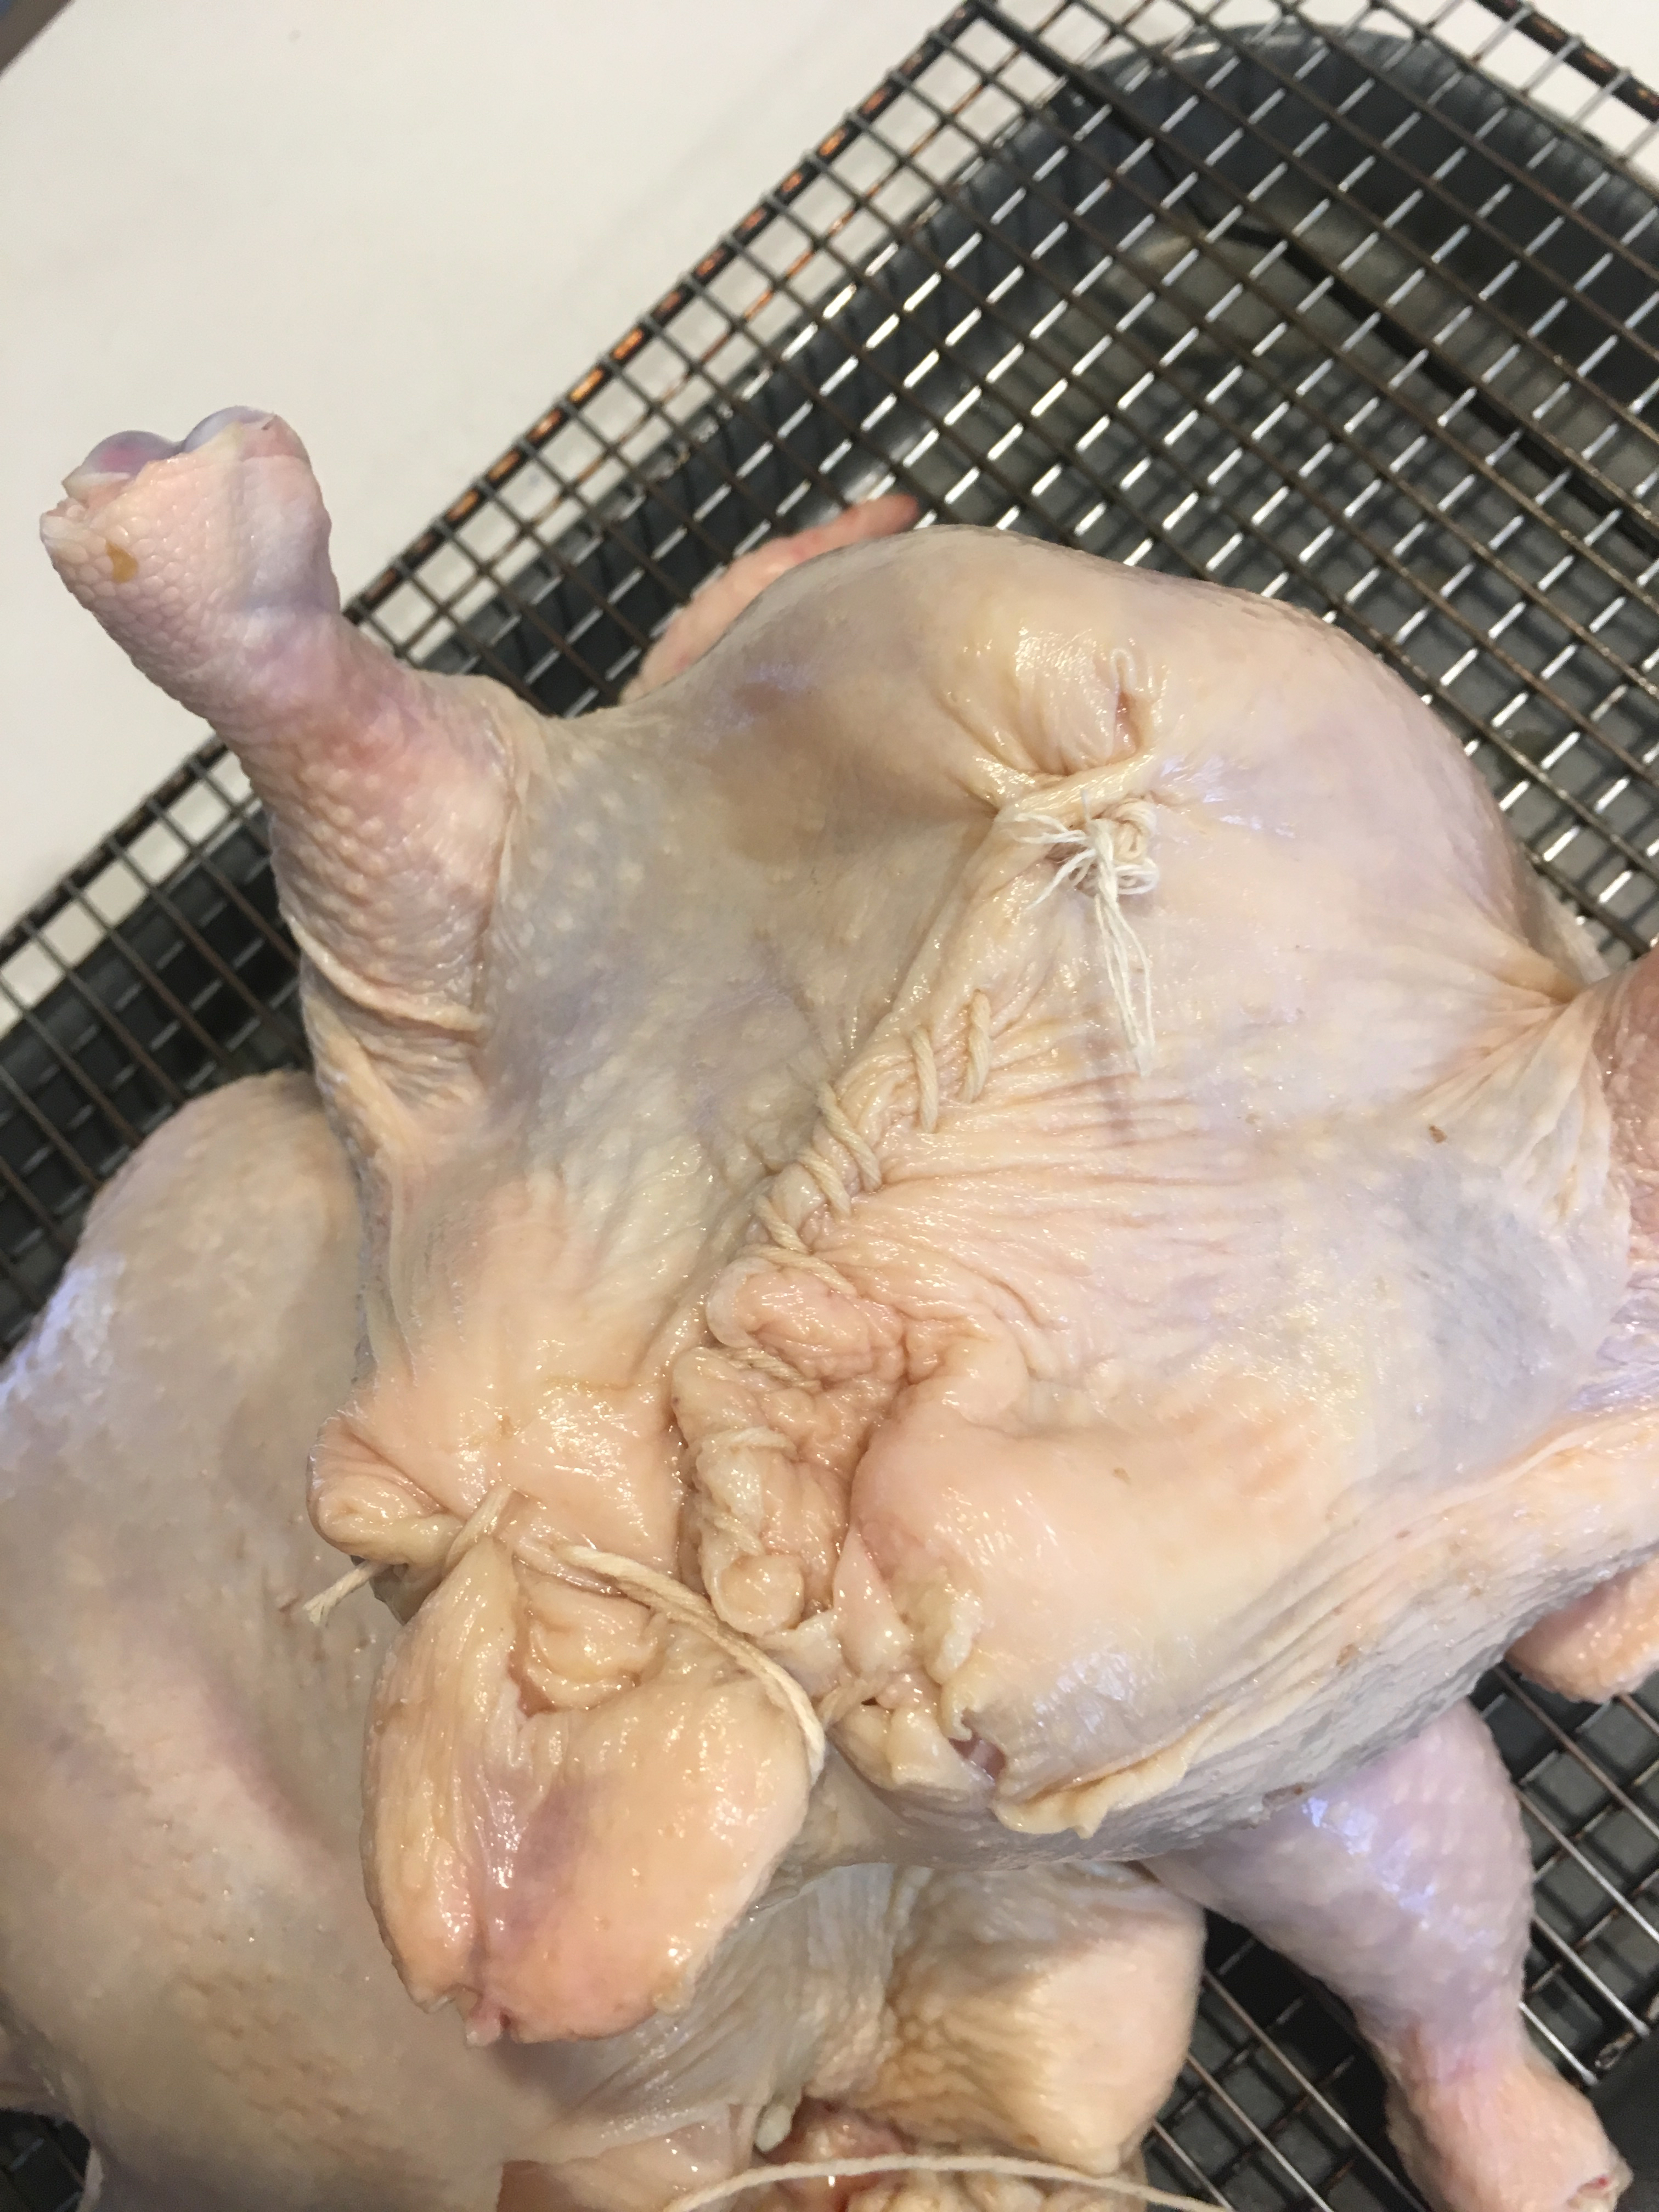
\includegraphics[width=0.25\textwidth]{\imageDir/\fileName/IMG_3217.jpg} &
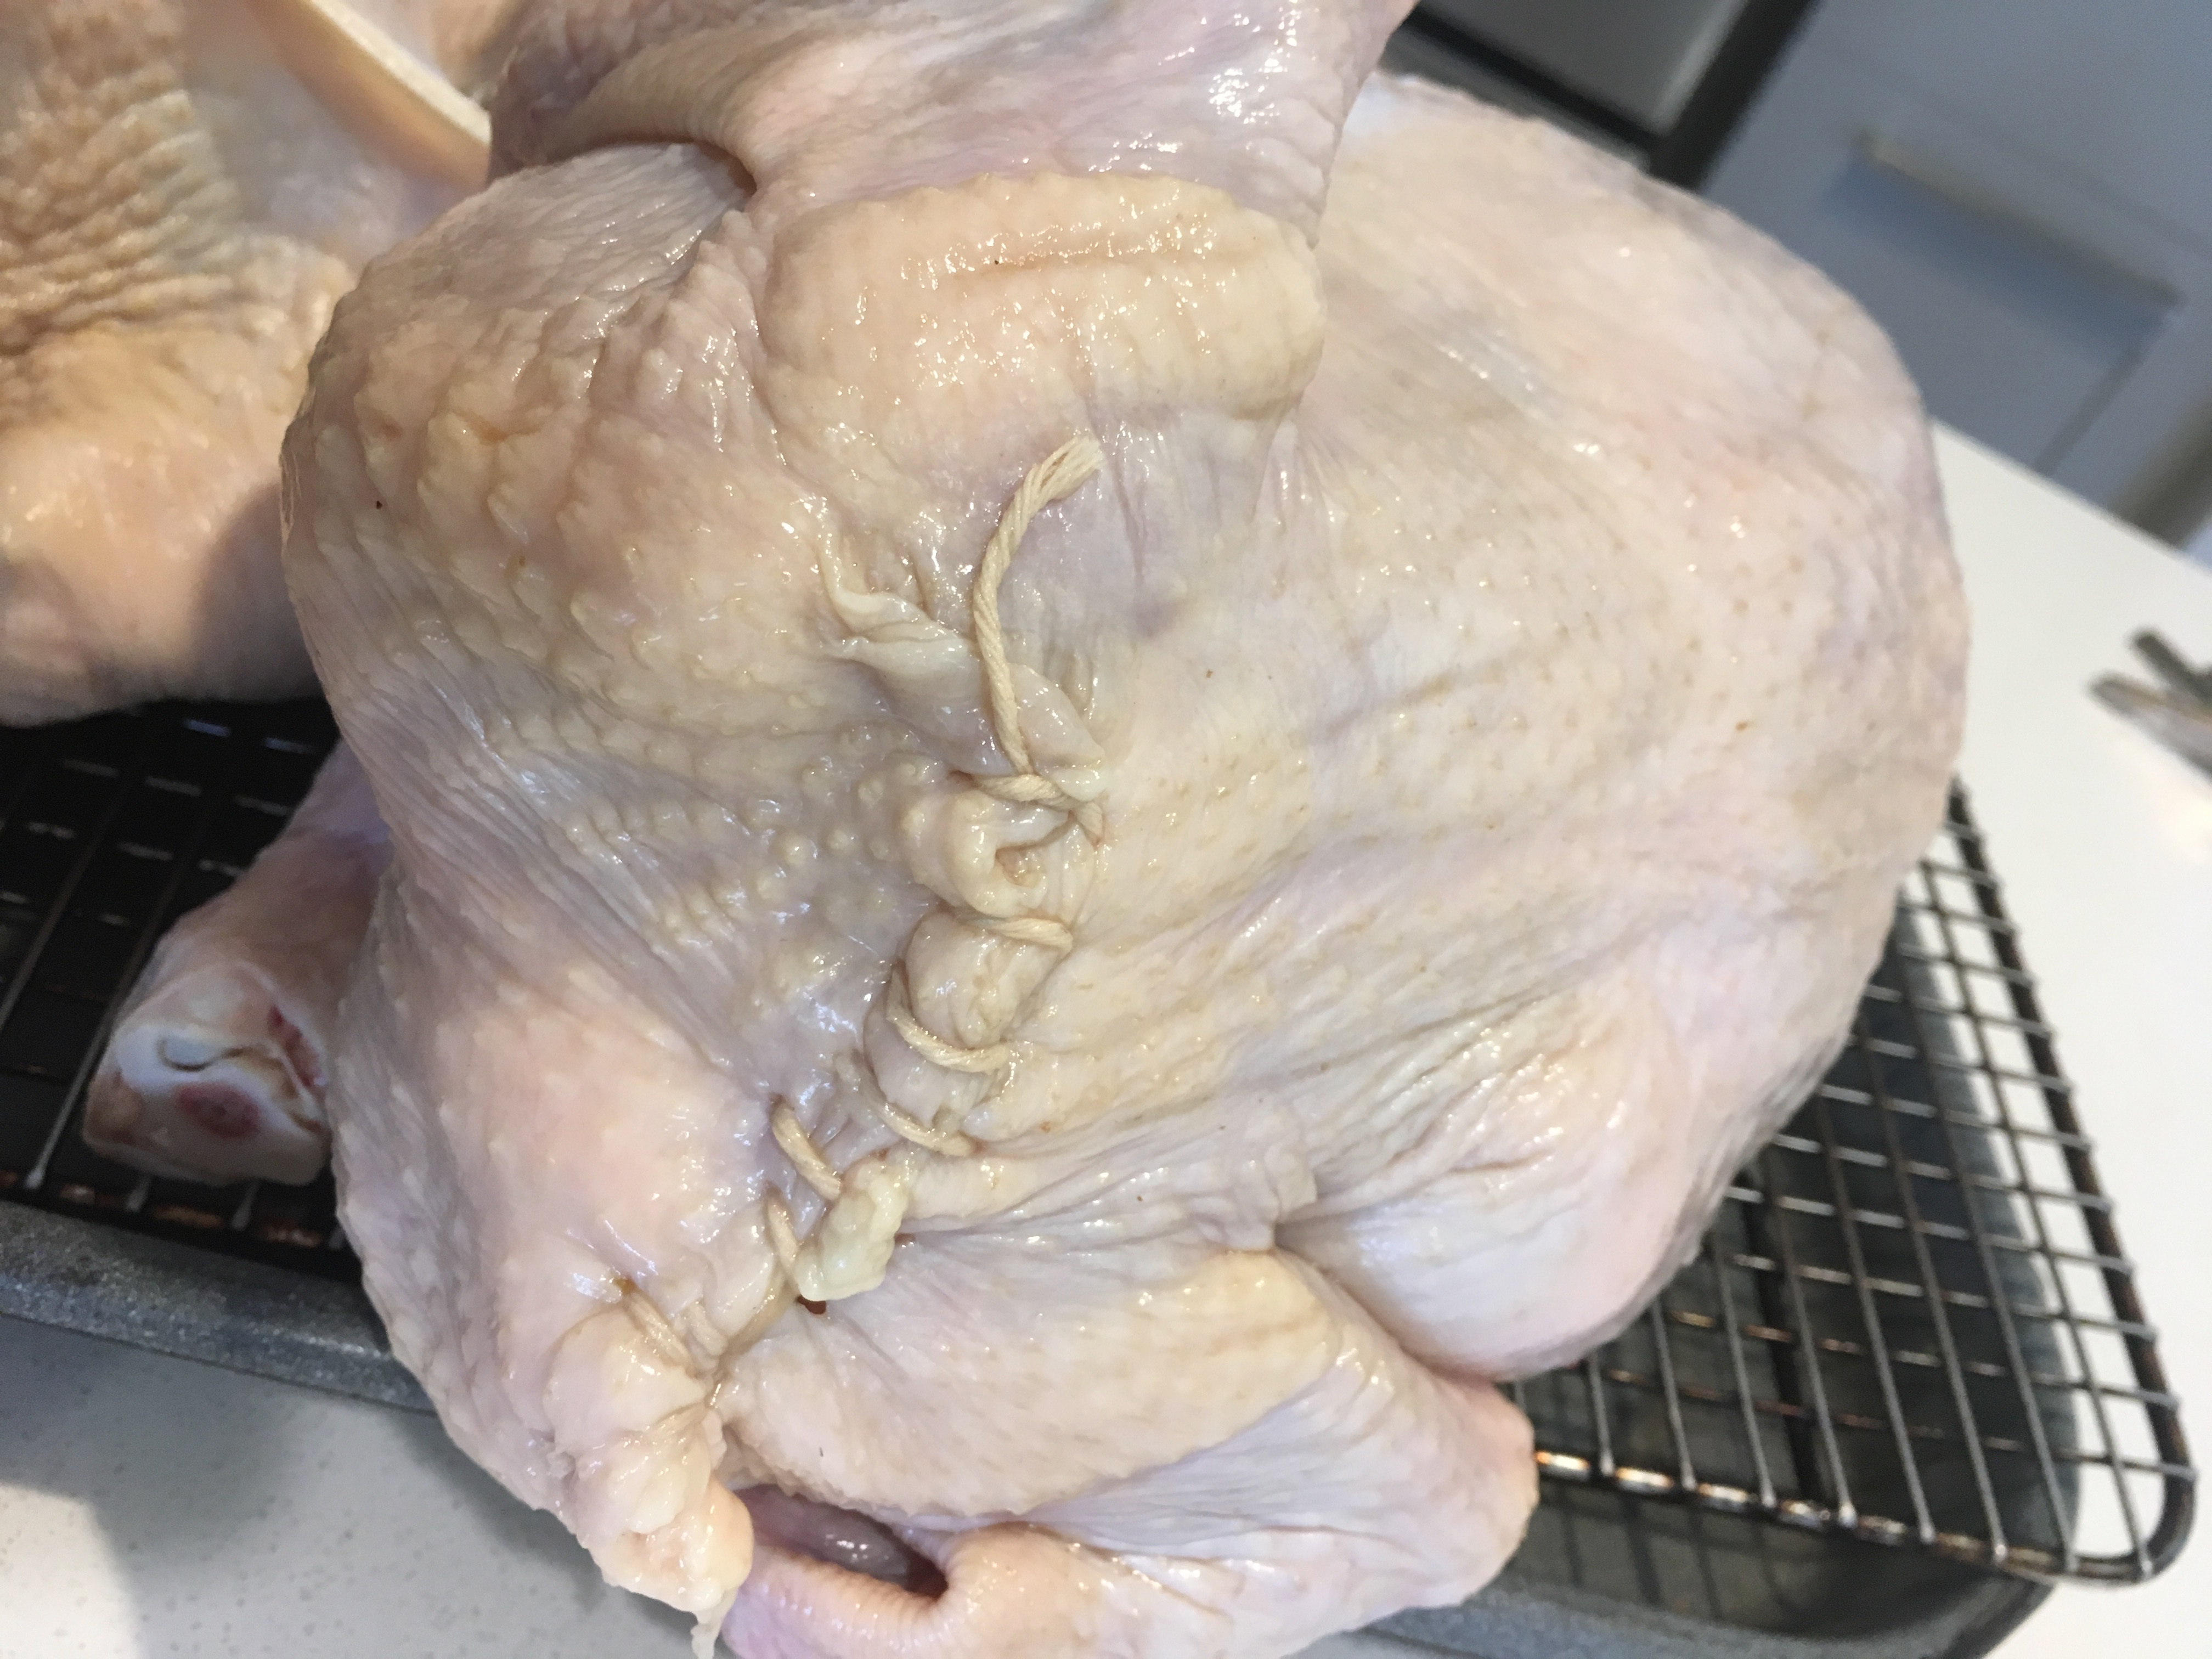
\includegraphics[width=0.25\textwidth]{\imageDir/\fileName/IMG_3218.jpg} &
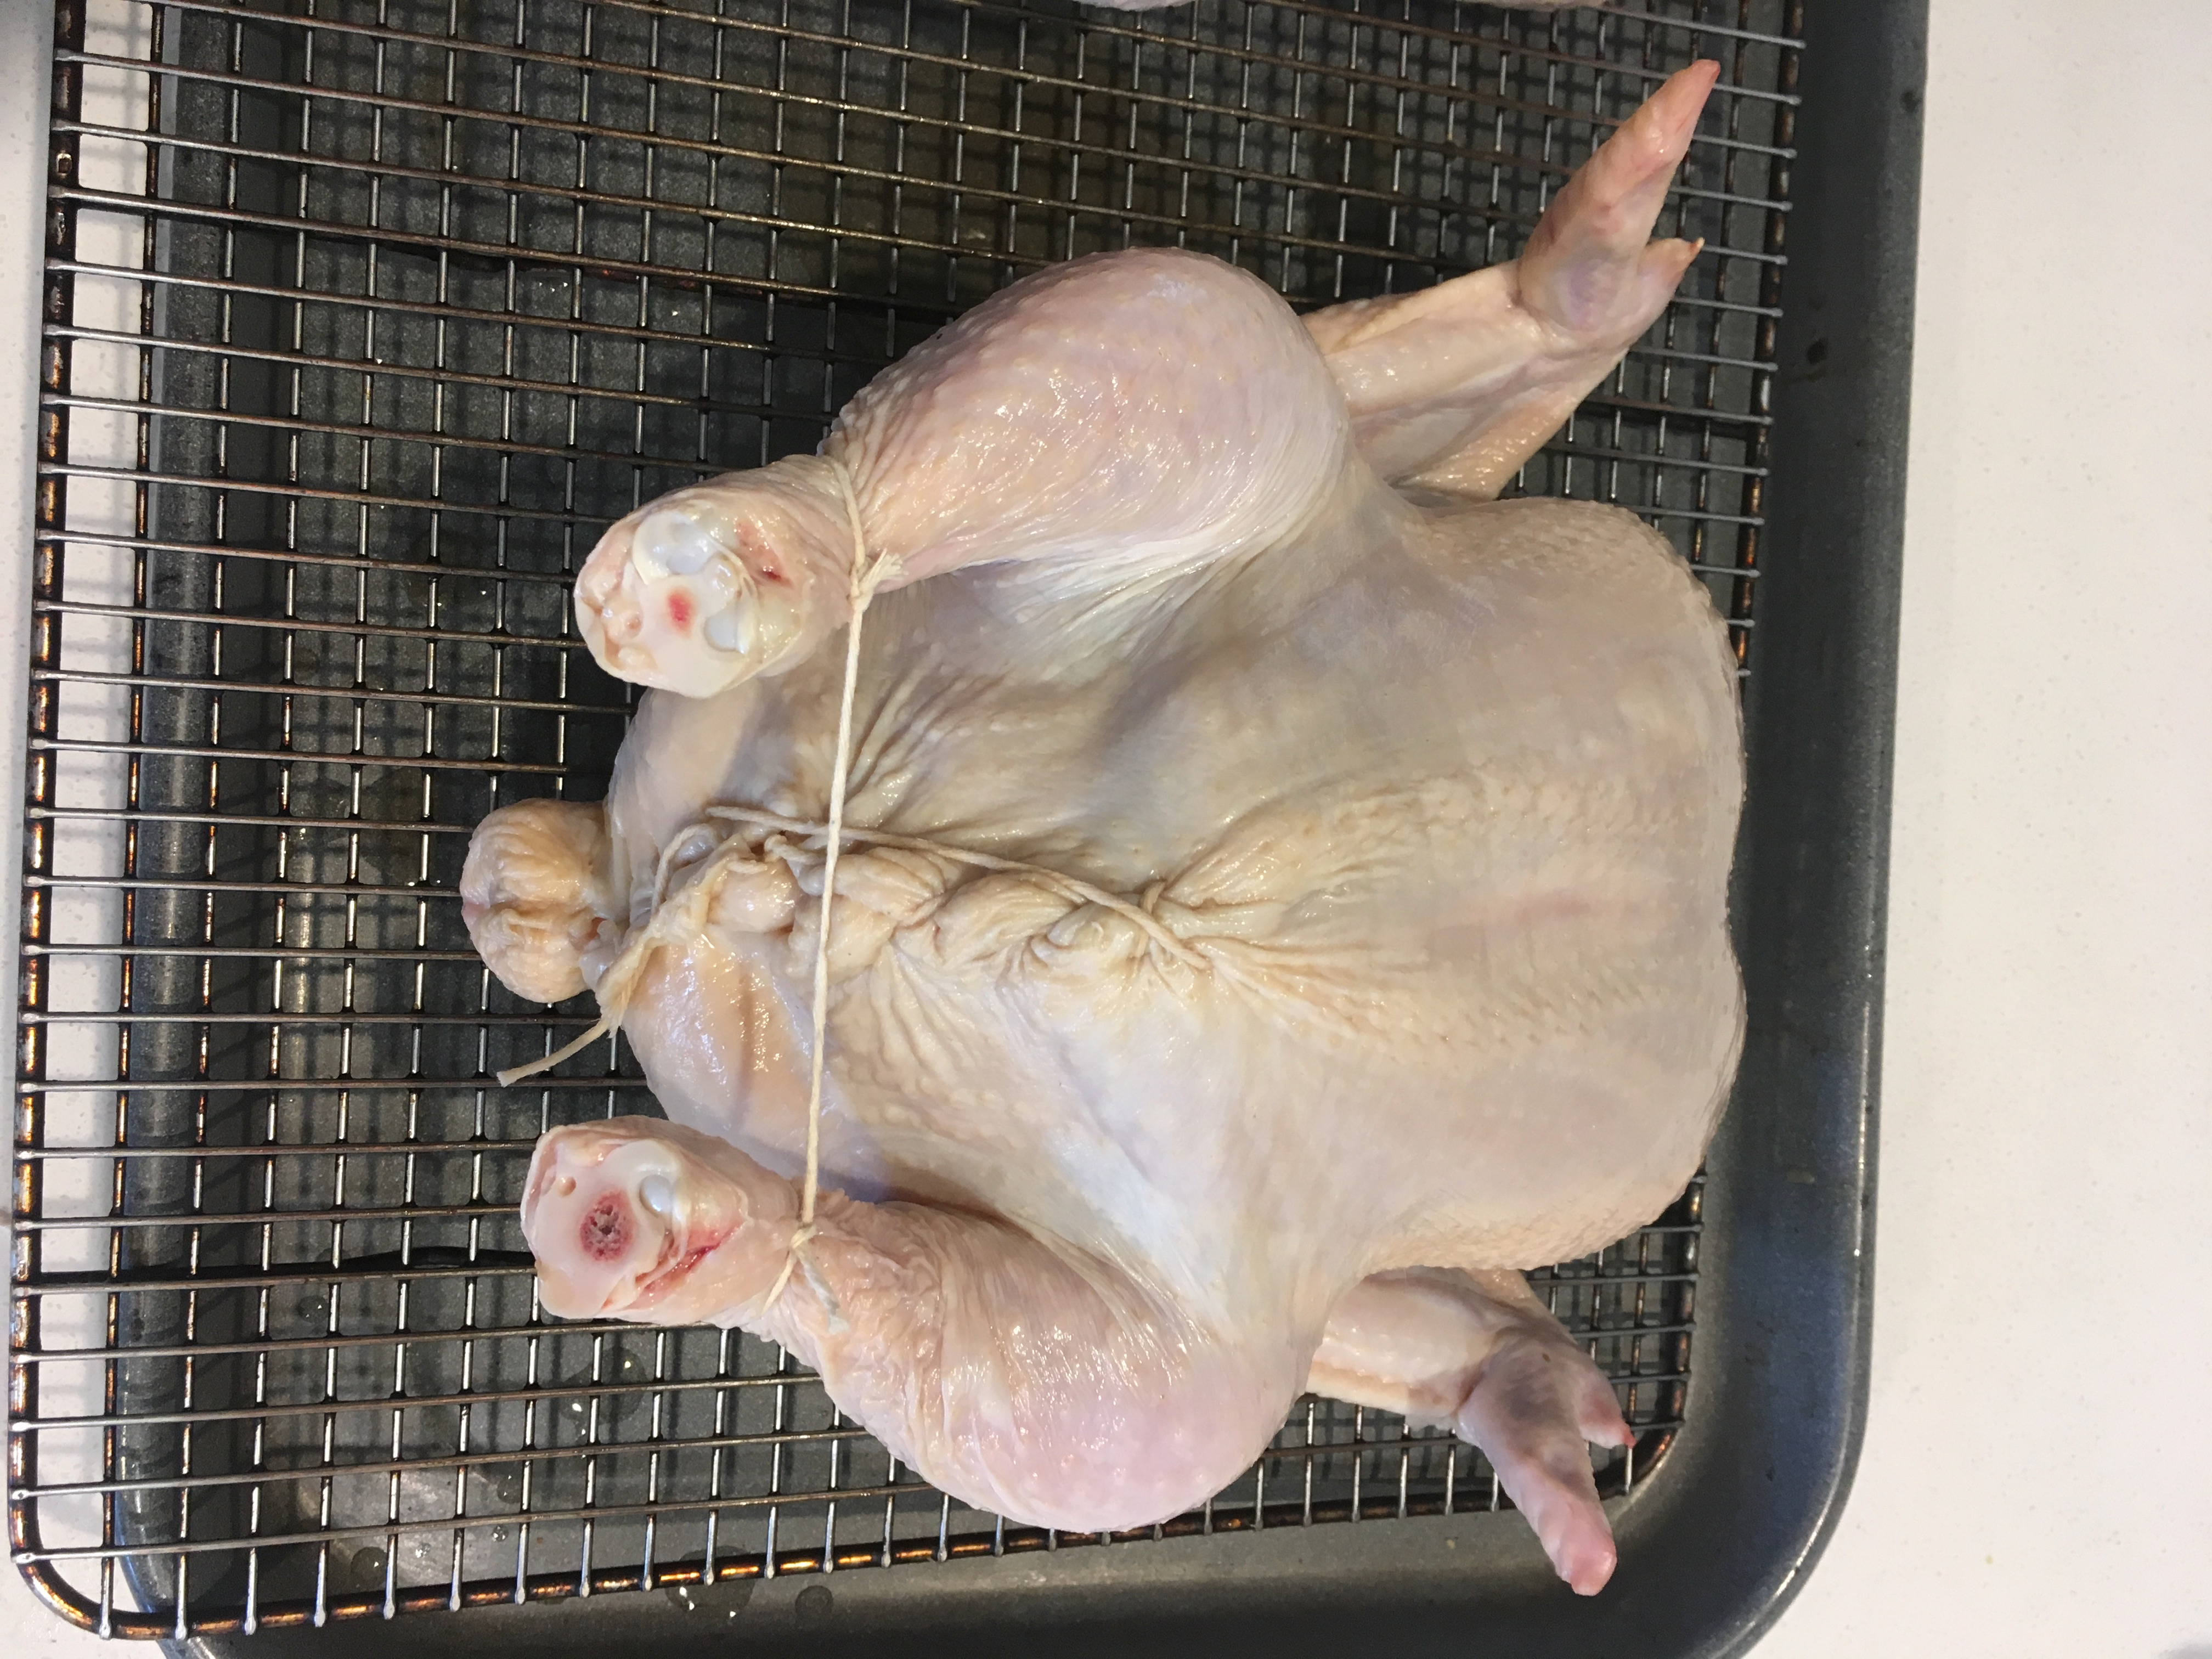
\includegraphics[width=0.25\textwidth]{\imageDir/\fileName/IMG_3219.jpg} \\
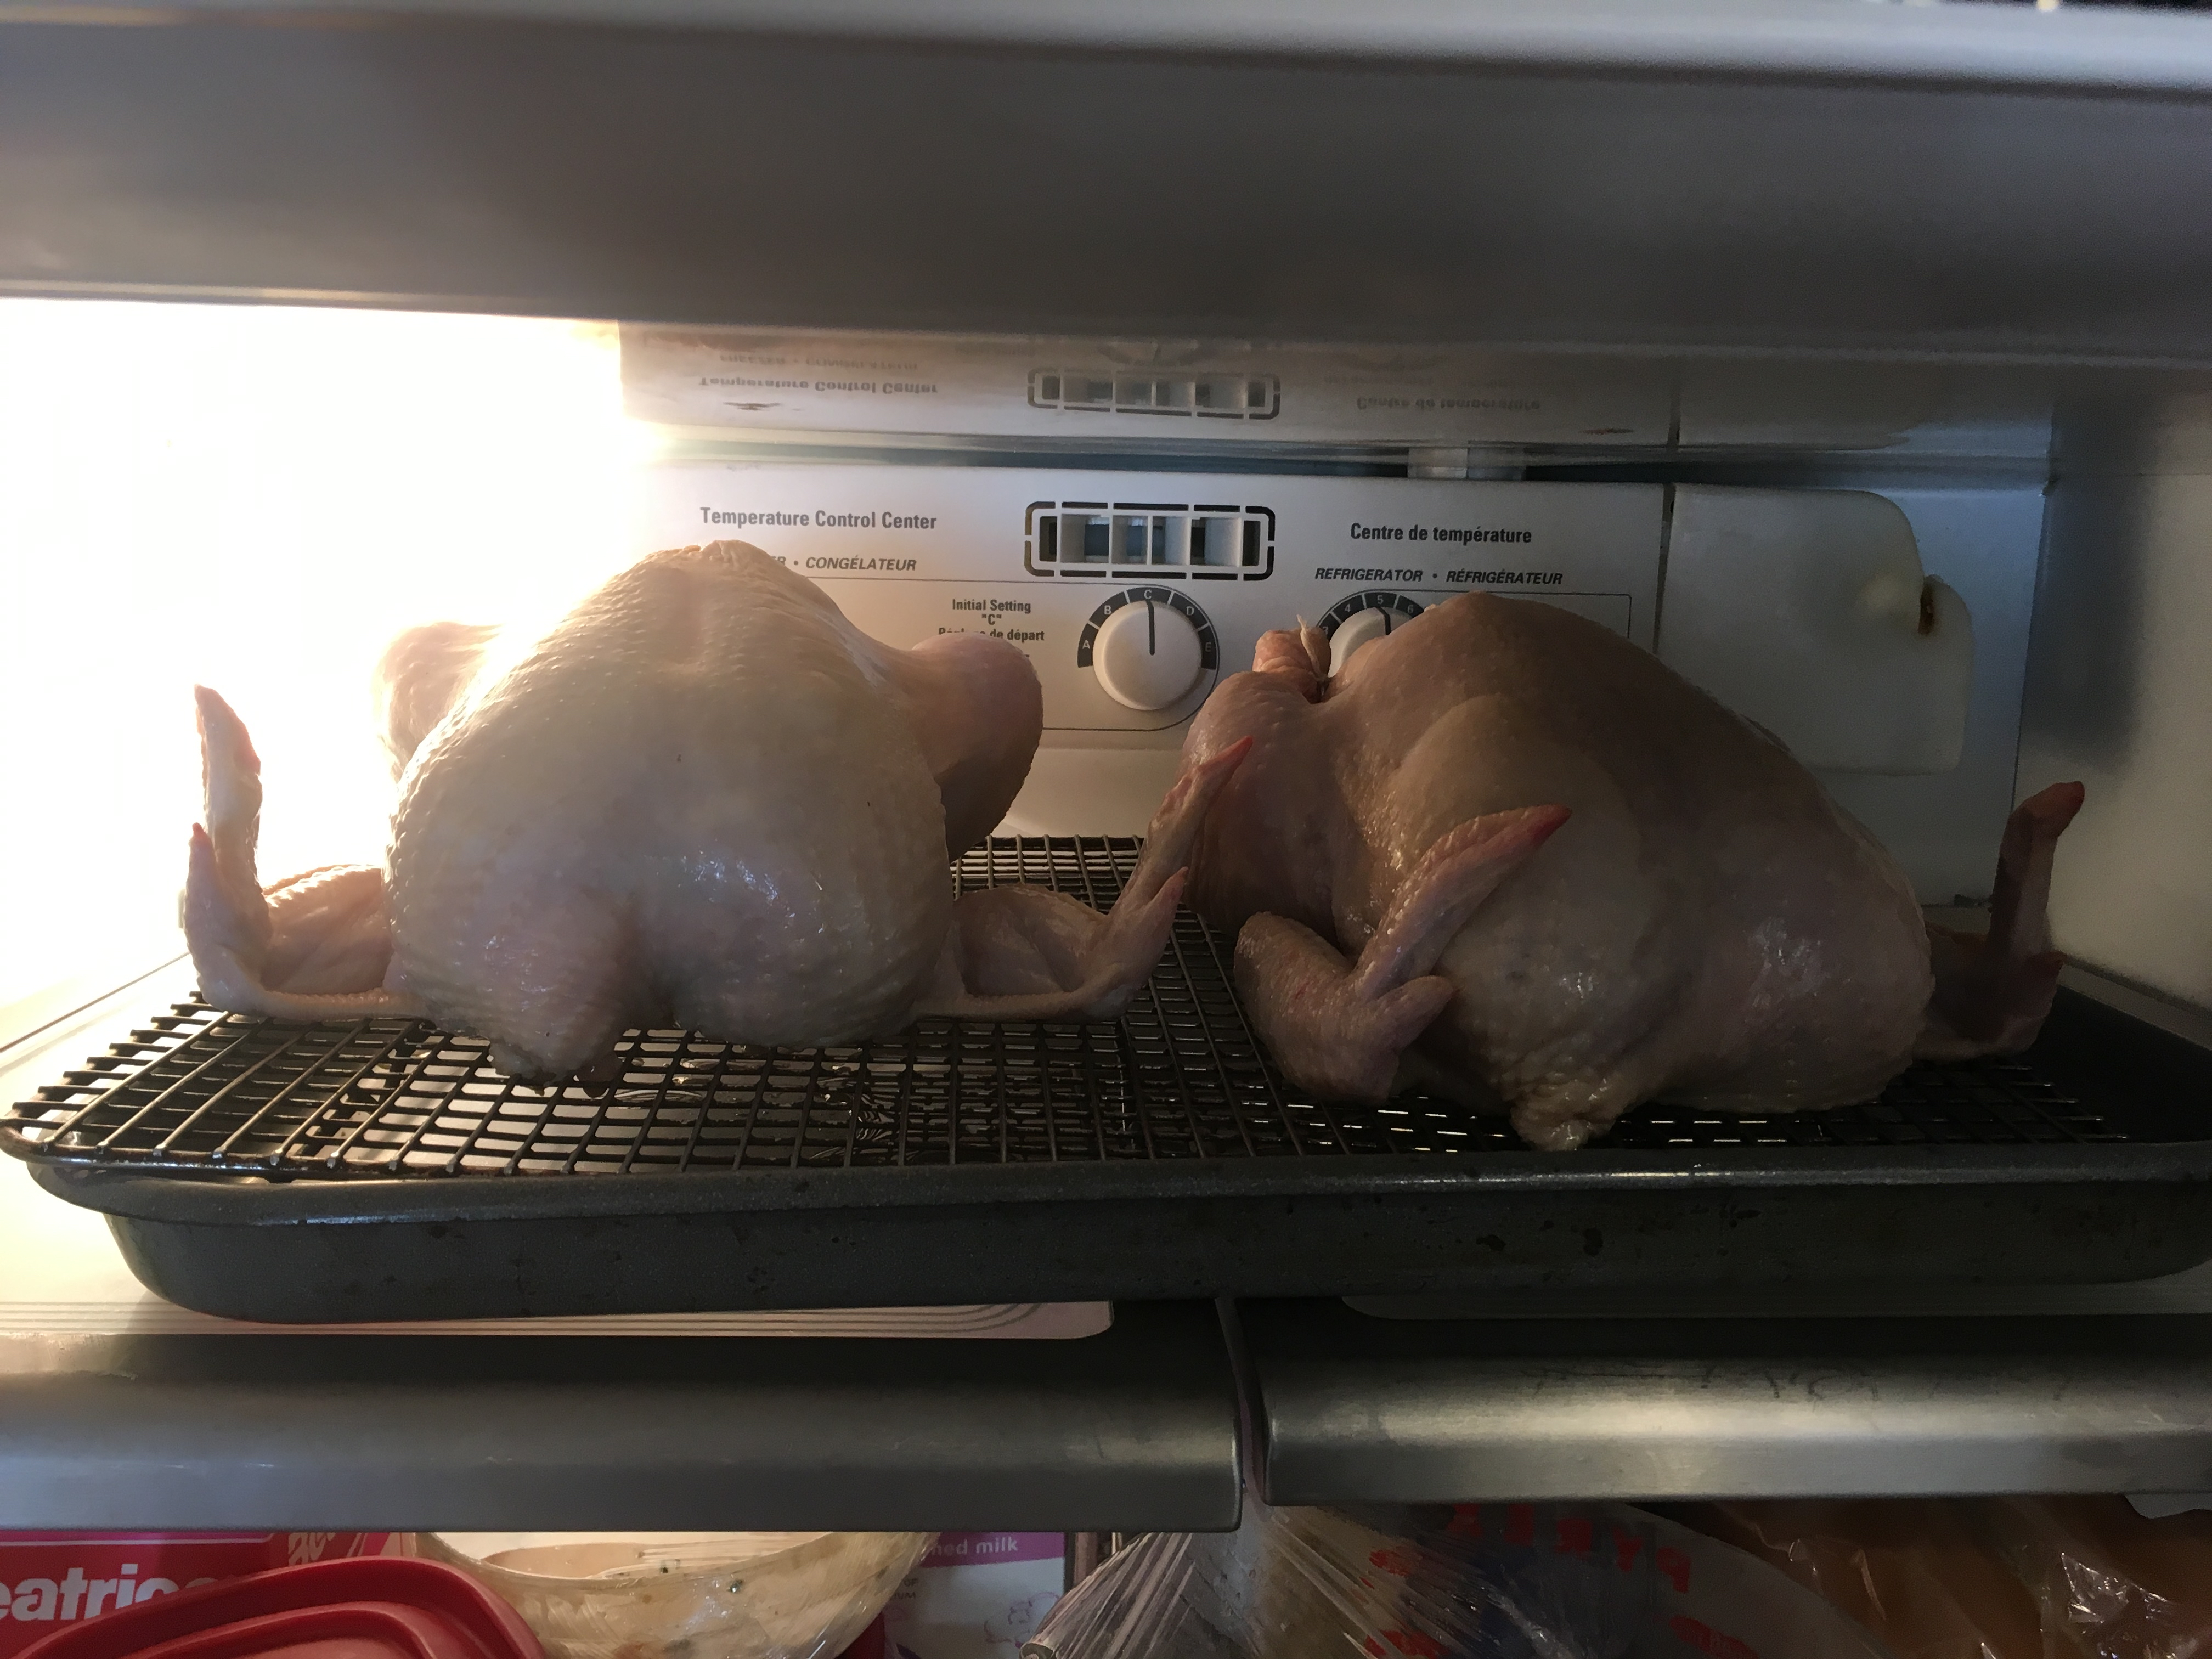
\includegraphics[width=0.25\textwidth]{\imageDir/\fileName/IMG_3220.jpg} &
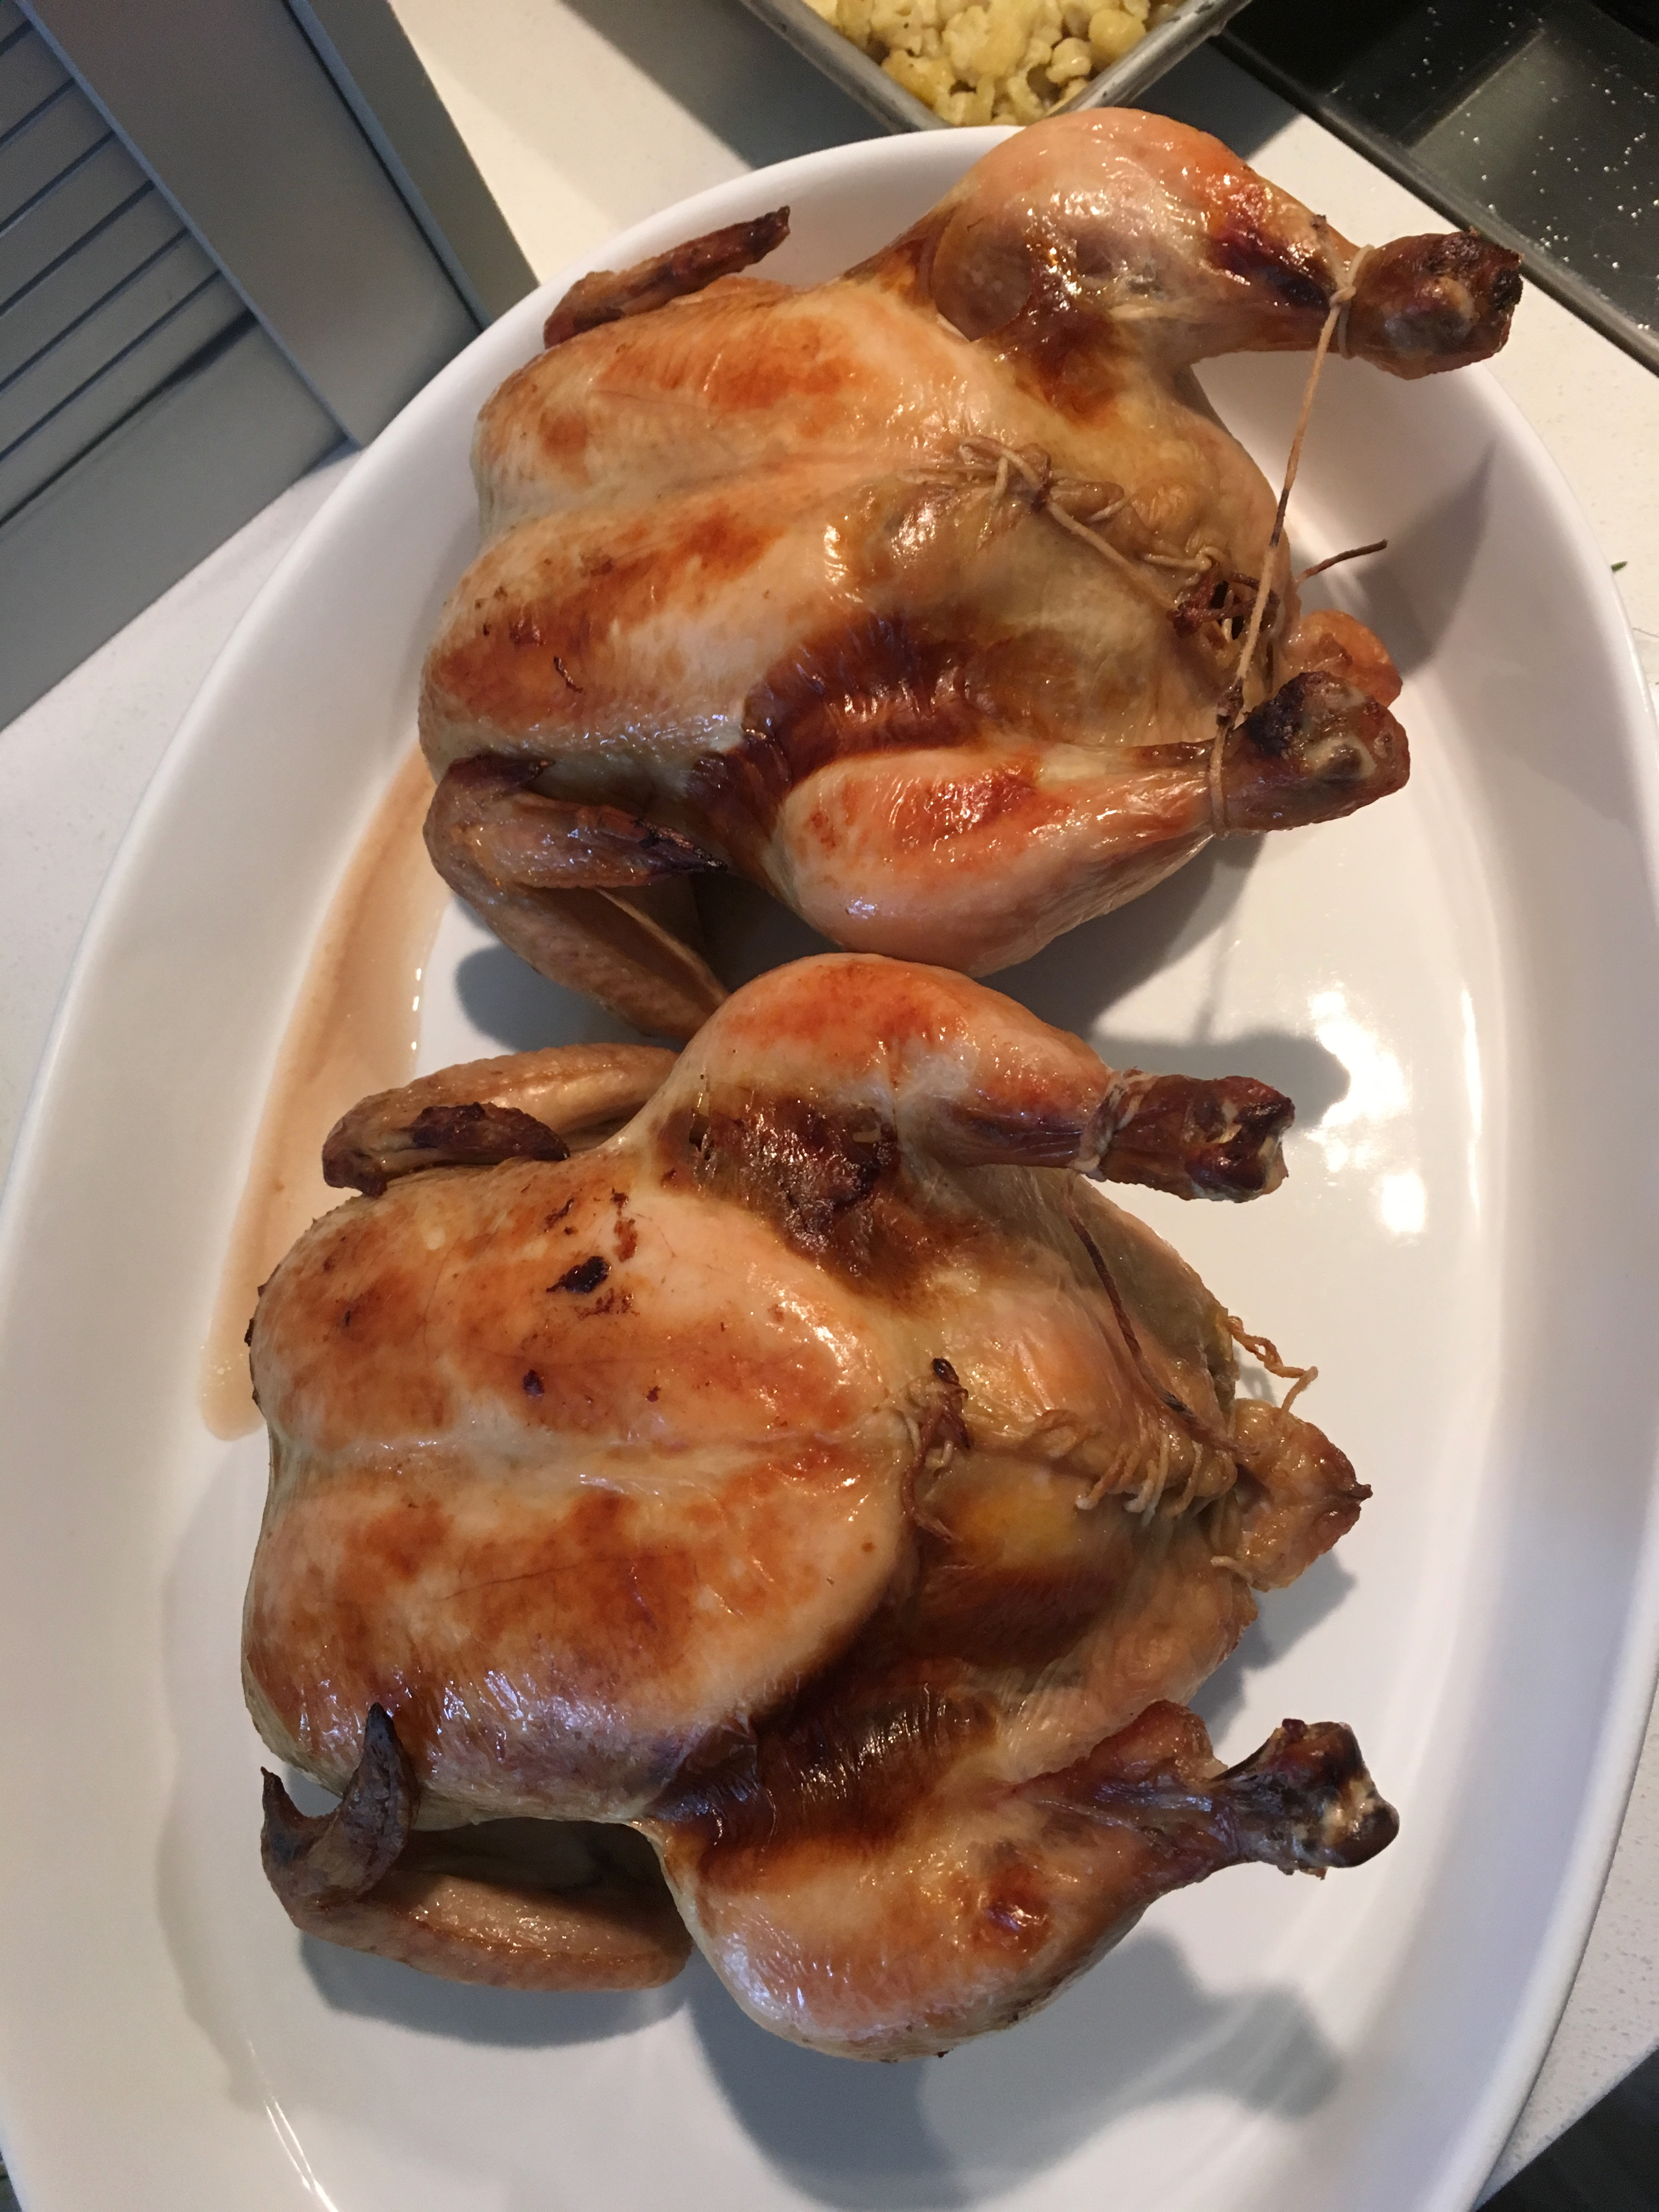
\includegraphics[width=0.25\textwidth]{\imageDir/\fileName/IMG_3228.jpg} \\
\end{tabular}
\end{table}

\end{document}
